\documentclass[twoside]{book}

% Packages required by doxygen
\usepackage{fixltx2e}
\usepackage{calc}
\usepackage{doxygen}
\usepackage{graphicx}
\usepackage[utf8]{inputenc}
\usepackage{makeidx}
\usepackage{multicol}
\usepackage{multirow}
\PassOptionsToPackage{warn}{textcomp}
\usepackage{textcomp}
\usepackage[nointegrals]{wasysym}
\usepackage[table]{xcolor}

% Font selection
\usepackage[T1]{fontenc}
\usepackage{mathptmx}
\usepackage[scaled=.90]{helvet}
\usepackage{courier}
\usepackage{amssymb}
\usepackage{sectsty}
\renewcommand{\familydefault}{\sfdefault}
\allsectionsfont{%
  \fontseries{bc}\selectfont%
  \color{darkgray}%
}
\renewcommand{\DoxyLabelFont}{%
  \fontseries{bc}\selectfont%
  \color{darkgray}%
}
\newcommand{\+}{\discretionary{\mbox{\scriptsize$\hookleftarrow$}}{}{}}

% Page & text layout
\usepackage{geometry}
\geometry{%
  a4paper,%
  top=2.5cm,%
  bottom=2.5cm,%
  left=2.5cm,%
  right=2.5cm%
}
\tolerance=750
\hfuzz=15pt
\hbadness=750
\setlength{\emergencystretch}{15pt}
\setlength{\parindent}{0cm}
\setlength{\parskip}{0.2cm}
\makeatletter
\renewcommand{\paragraph}{%
  \@startsection{paragraph}{4}{0ex}{-1.0ex}{1.0ex}{%
    \normalfont\normalsize\bfseries\SS@parafont%
  }%
}
\renewcommand{\subparagraph}{%
  \@startsection{subparagraph}{5}{0ex}{-1.0ex}{1.0ex}{%
    \normalfont\normalsize\bfseries\SS@subparafont%
  }%
}
\makeatother

% Headers & footers
\usepackage{fancyhdr}
\pagestyle{fancyplain}
\fancyhead[LE]{\fancyplain{}{\bfseries\thepage}}
\fancyhead[CE]{\fancyplain{}{}}
\fancyhead[RE]{\fancyplain{}{\bfseries\leftmark}}
\fancyhead[LO]{\fancyplain{}{\bfseries\rightmark}}
\fancyhead[CO]{\fancyplain{}{}}
\fancyhead[RO]{\fancyplain{}{\bfseries\thepage}}
\fancyfoot[LE]{\fancyplain{}{}}
\fancyfoot[CE]{\fancyplain{}{}}
\fancyfoot[RE]{\fancyplain{}{\bfseries\scriptsize Generated on Sun Jun 15 2014 16\+:41\+:34 for Projet L\+O21 by Doxygen }}
\fancyfoot[LO]{\fancyplain{}{\bfseries\scriptsize Generated on Sun Jun 15 2014 16\+:41\+:34 for Projet L\+O21 by Doxygen }}
\fancyfoot[CO]{\fancyplain{}{}}
\fancyfoot[RO]{\fancyplain{}{}}
\renewcommand{\footrulewidth}{0.4pt}
\renewcommand{\chaptermark}[1]{%
  \markboth{#1}{}%
}
\renewcommand{\sectionmark}[1]{%
  \markright{\thesection\ #1}%
}

% Indices & bibliography
\usepackage{natbib}
\usepackage[titles]{tocloft}
\setcounter{tocdepth}{3}
\setcounter{secnumdepth}{5}
\makeindex

% Hyperlinks (required, but should be loaded last)
\usepackage{ifpdf}
\ifpdf
  \usepackage[pdftex,pagebackref=true]{hyperref}
\else
  \usepackage[ps2pdf,pagebackref=true]{hyperref}
\fi
\hypersetup{%
  colorlinks=true,%
  linkcolor=blue,%
  citecolor=blue,%
  unicode%
}

% Custom commands
\newcommand{\clearemptydoublepage}{%
  \newpage{\pagestyle{empty}\cleardoublepage}%
}


%===== C O N T E N T S =====

\begin{document}

% Titlepage & ToC
\hypersetup{pageanchor=false,
             bookmarks=true,
             bookmarksnumbered=true,
             pdfencoding=unicode
            }
\pagenumbering{roman}
\begin{titlepage}
\vspace*{7cm}
\begin{center}%
{\Large Projet L\+O21 }\\
\vspace*{1cm}
{\large Generated by Doxygen 1.8.7}\\
\vspace*{0.5cm}
{\small Sun Jun 15 2014 16:41:34}\\
\end{center}
\end{titlepage}
\clearemptydoublepage
\tableofcontents
\clearemptydoublepage
\pagenumbering{arabic}
\hypersetup{pageanchor=true}

%--- Begin generated contents ---
\chapter{Hierarchical Index}
\section{Class Hierarchy}
This inheritance list is sorted roughly, but not completely, alphabetically\+:\begin{DoxyCompactList}
\item \contentsline{section}{Etudiant}{\pageref{classEtudiant}}{}
\item exception\begin{DoxyCompactList}
\item \contentsline{section}{semestre\+Invalide\+Erreur}{\pageref{classsemestreInvalideErreur}}{}
\end{DoxyCompactList}
\item Q\+Dialog\begin{DoxyCompactList}
\item \contentsline{section}{Q\+Semestre\+Dialog}{\pageref{classQSemestreDialog}}{}
\item \contentsline{section}{Q\+User\+Dialog}{\pageref{classQUserDialog}}{}
\end{DoxyCompactList}
\item Q\+Layout\begin{DoxyCompactList}
\item \contentsline{section}{Flow\+Layout}{\pageref{classFlowLayout}}{}
\end{DoxyCompactList}
\item Q\+Main\+Window\begin{DoxyCompactList}
\item \contentsline{section}{Main\+Window}{\pageref{classMainWindow}}{}
\end{DoxyCompactList}
\item Q\+Object\begin{DoxyCompactList}
\item \contentsline{section}{Formation\+Controller}{\pageref{classFormationController}}{}
\item \contentsline{section}{Main\+Window\+Controller}{\pageref{classMainWindowController}}{}
\item \contentsline{section}{Semestre\+Controller}{\pageref{classSemestreController}}{}
\item \contentsline{section}{Semestre\+Dialog\+Controller}{\pageref{classSemestreDialogController}}{}
\item \contentsline{section}{U\+V\+Choisie\+Controller}{\pageref{classUVChoisieController}}{}
\end{DoxyCompactList}
\item Q\+Standard\+Item\+Model\begin{DoxyCompactList}
\item \contentsline{section}{Q\+U\+V\+List\+Item\+Model}{\pageref{classQUVListItemModel}}{}
\end{DoxyCompactList}
\item Q\+Widget\begin{DoxyCompactList}
\item \contentsline{section}{Q\+Filtre\+Branche}{\pageref{classQFiltreBranche}}{}
\item \contentsline{section}{Q\+Formation}{\pageref{classQFormation}}{}
\item \contentsline{section}{Q\+Semestre}{\pageref{classQSemestre}}{}
\item \contentsline{section}{Q\+U\+V\+Choisie}{\pageref{classQUVChoisie}}{}
\item \contentsline{section}{Q\+U\+V\+Preview}{\pageref{classQUVPreview}}{}
\end{DoxyCompactList}
\item \contentsline{section}{Xml\+Convertible}{\pageref{classXmlConvertible}}{}
\begin{DoxyCompactList}
\item \contentsline{section}{Catalogue}{\pageref{classCatalogue}}{}
\item \contentsline{section}{Formation}{\pageref{classFormation}}{}
\begin{DoxyCompactList}
\item \contentsline{section}{Formation\+Hors\+Utc}{\pageref{classFormationHorsUtc}}{}
\item \contentsline{section}{Formation\+Utc}{\pageref{classFormationUtc}}{}
\end{DoxyCompactList}
\item \contentsline{section}{Semestre}{\pageref{classSemestre}}{}
\item \contentsline{section}{U\+V}{\pageref{classUV}}{}
\item \contentsline{section}{U\+V\+Etudiant}{\pageref{classUVEtudiant}}{}
\end{DoxyCompactList}
\end{DoxyCompactList}

\chapter{Class Index}
\section{Class List}
Here are the classes, structs, unions and interfaces with brief descriptions\+:\begin{DoxyCompactList}
\item\contentsline{section}{\hyperlink{classCatalogue}{Catalogue} }{\pageref{classCatalogue}}{}
\item\contentsline{section}{\hyperlink{classEtudiant}{Etudiant} }{\pageref{classEtudiant}}{}
\item\contentsline{section}{\hyperlink{classFlowLayout}{Flow\+Layout} }{\pageref{classFlowLayout}}{}
\item\contentsline{section}{\hyperlink{classFormation}{Formation} }{\pageref{classFormation}}{}
\item\contentsline{section}{\hyperlink{classFormationController}{Formation\+Controller} }{\pageref{classFormationController}}{}
\item\contentsline{section}{\hyperlink{classFormationHorsUtc}{Formation\+Hors\+Utc} }{\pageref{classFormationHorsUtc}}{}
\item\contentsline{section}{\hyperlink{classFormationUtc}{Formation\+Utc} }{\pageref{classFormationUtc}}{}
\item\contentsline{section}{\hyperlink{classMainWindow}{Main\+Window} }{\pageref{classMainWindow}}{}
\item\contentsline{section}{\hyperlink{classMainWindowController}{Main\+Window\+Controller} }{\pageref{classMainWindowController}}{}
\item\contentsline{section}{\hyperlink{classQFiltreBranche}{Q\+Filtre\+Branche} }{\pageref{classQFiltreBranche}}{}
\item\contentsline{section}{\hyperlink{classQFormation}{Q\+Formation} }{\pageref{classQFormation}}{}
\item\contentsline{section}{\hyperlink{classQSemestre}{Q\+Semestre} }{\pageref{classQSemestre}}{}
\item\contentsline{section}{\hyperlink{classQSemestreDialog}{Q\+Semestre\+Dialog} }{\pageref{classQSemestreDialog}}{}
\item\contentsline{section}{\hyperlink{classQUserDialog}{Q\+User\+Dialog} }{\pageref{classQUserDialog}}{}
\item\contentsline{section}{\hyperlink{classQUVChoisie}{Q\+U\+V\+Choisie} }{\pageref{classQUVChoisie}}{}
\item\contentsline{section}{\hyperlink{classQUVListItemModel}{Q\+U\+V\+List\+Item\+Model} }{\pageref{classQUVListItemModel}}{}
\item\contentsline{section}{\hyperlink{classQUVPreview}{Q\+U\+V\+Preview} }{\pageref{classQUVPreview}}{}
\item\contentsline{section}{\hyperlink{classSemestre}{Semestre} }{\pageref{classSemestre}}{}
\item\contentsline{section}{\hyperlink{classSemestreController}{Semestre\+Controller} }{\pageref{classSemestreController}}{}
\item\contentsline{section}{\hyperlink{classSemestreDialogController}{Semestre\+Dialog\+Controller} }{\pageref{classSemestreDialogController}}{}
\item\contentsline{section}{\hyperlink{classsemestreInvalideErreur}{semestre\+Invalide\+Erreur} }{\pageref{classsemestreInvalideErreur}}{}
\item\contentsline{section}{\hyperlink{classUV}{U\+V} }{\pageref{classUV}}{}
\item\contentsline{section}{\hyperlink{classUVChoisieController}{U\+V\+Choisie\+Controller} }{\pageref{classUVChoisieController}}{}
\item\contentsline{section}{\hyperlink{classUVEtudiant}{U\+V\+Etudiant} }{\pageref{classUVEtudiant}}{}
\item\contentsline{section}{\hyperlink{classXmlConvertible}{Xml\+Convertible} }{\pageref{classXmlConvertible}}{}
\end{DoxyCompactList}

\chapter{Class Documentation}
\hypertarget{classCatalogue}{\section{Catalogue Class Reference}
\label{classCatalogue}\index{Catalogue@{Catalogue}}
}
Inheritance diagram for Catalogue\+:\begin{figure}[H]
\begin{center}
\leavevmode
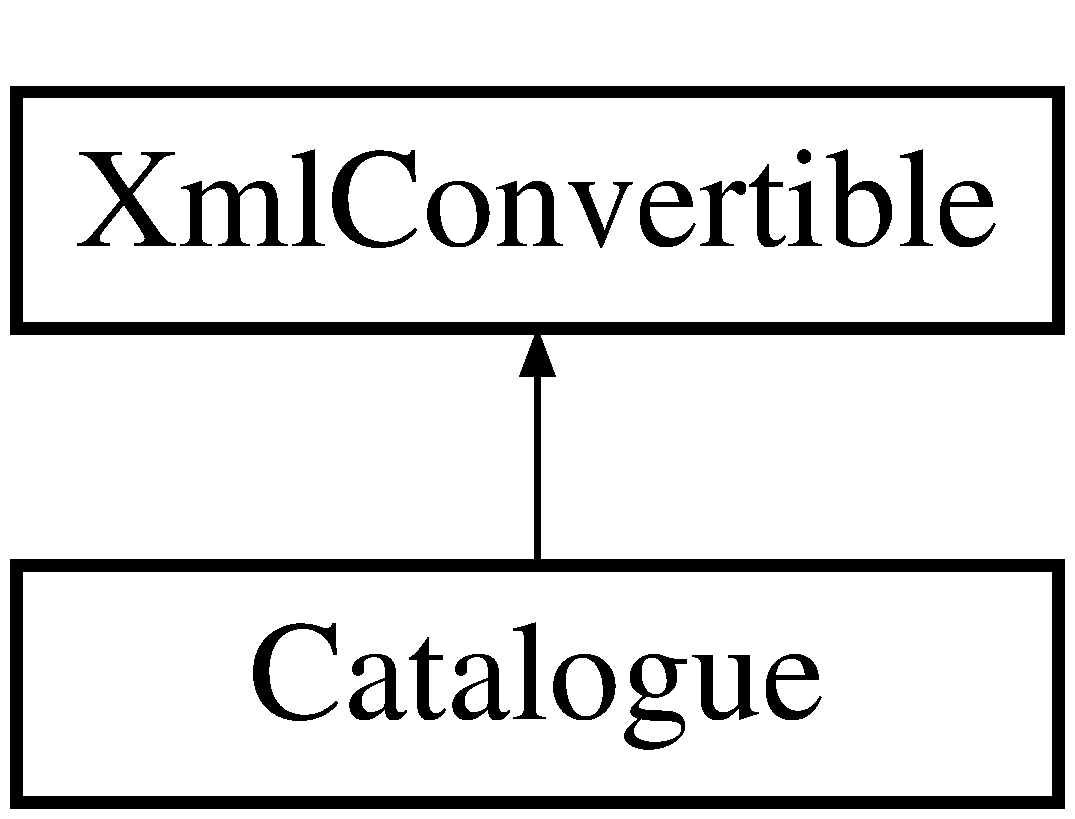
\includegraphics[height=2.000000cm]{classCatalogue}
\end{center}
\end{figure}
\subsection*{Public Member Functions}
\begin{DoxyCompactItemize}
\item 
\hyperlink{classUV}{U\+V} $\ast$ \hyperlink{classCatalogue_a0b41015c9bdedce5463c077e4f5911d9}{operator\mbox{[}$\,$\mbox{]}} (Q\+String tag)
\item 
const \hyperlink{classUV}{U\+V} $\ast$ \hyperlink{classCatalogue_ad3c0bd9f62e5dfac1793a38b28b0eb7d}{operator\mbox{[}$\,$\mbox{]}} (Q\+String tag) const 
\item 
void \hyperlink{classCatalogue_aaa115ae803e70505a8c1973dc77ed16e}{ajouter\+Uv} (\hyperlink{classUV}{U\+V} $\ast$uv)
\begin{DoxyCompactList}\small\item\em Ajoute une uv au catalogue. \end{DoxyCompactList}\item 
void \hyperlink{classCatalogue_aac46b55131756fab4116334f40e2db08}{supprimer\+Uv} (const Q\+String uv)
\begin{DoxyCompactList}\small\item\em Supprime une uv du catalogue. \end{DoxyCompactList}\item 
void \hyperlink{classCatalogue_ad57d112222cd659ce25e4c1f2a656a37}{editer\+Uv} (const Q\+String old\+Tag, \hyperlink{classUV}{U\+V} $\ast$uv)
\begin{DoxyCompactList}\small\item\em Edite une uv du catalogue. \end{DoxyCompactList}\item 
bool \hyperlink{classCatalogue_aa09bcaa689f5c1a99b2938eb207fcb53}{existe} (Q\+String tag)
\item 
\hypertarget{classCatalogue_a5041850ff2105de5cc0a60bd81428f29}{void {\bfseries sauvegarder} ()}\label{classCatalogue_a5041850ff2105de5cc0a60bd81428f29}

\item 
\hypertarget{classCatalogue_a0a8e893d0f54ca2ce1583758c5b6cf05}{void \hyperlink{classCatalogue_a0a8e893d0f54ca2ce1583758c5b6cf05}{from\+Xml} (const Q\+Dom\+Node \&noeud)}\label{classCatalogue_a0a8e893d0f54ca2ce1583758c5b6cf05}

\begin{DoxyCompactList}\small\item\em Définit l'objet à partir d'un élément X\+M\+L. \end{DoxyCompactList}\item 
Q\+Dom\+Element \hyperlink{classCatalogue_a12f412e8ba3dd8b950fc1f7dd8608f51}{to\+Xml} () const 
\begin{DoxyCompactList}\small\item\em Convertit l'objet au format X\+M\+L. \end{DoxyCompactList}\item 
\hypertarget{classCatalogue_ad474a13f9542c20894560310b75f431c}{Q\+Set$<$ Q\+String $>$ {\bfseries cursus} () const }\label{classCatalogue_ad474a13f9542c20894560310b75f431c}

\item 
\hypertarget{classCatalogue_a262a14d33cd2d6d8192a2b00b15cdb7f}{Q\+Map$<$ Q\+String, \hyperlink{classUV}{U\+V} $\ast$ $>$ {\bfseries uvs} () const }\label{classCatalogue_a262a14d33cd2d6d8192a2b00b15cdb7f}

\item 
\hypertarget{classCatalogue_a5992f2acc3cec15b819b97b1f36303ad}{Q\+String {\bfseries to\+String} ()}\label{classCatalogue_a5992f2acc3cec15b819b97b1f36303ad}

\end{DoxyCompactItemize}
\subsection*{Static Public Member Functions}
\begin{DoxyCompactItemize}
\item 
static const \hyperlink{classCatalogue}{Catalogue} $\ast$ \hyperlink{classCatalogue_a875a4bd0a28d97b500b5d67704f273a6}{instance} ()
\end{DoxyCompactItemize}
\subsection*{Static Public Attributes}
\begin{DoxyCompactItemize}
\item 
\hypertarget{classCatalogue_a068d1f58e7854f79b05a30667dfebc32}{static const Q\+String \hyperlink{classCatalogue_a068d1f58e7854f79b05a30667dfebc32}{X\+M\+L\+\_\+\+N\+O\+D\+E\+\_\+\+N\+A\+M\+E} = \char`\"{}catalogue\char`\"{}}\label{classCatalogue_a068d1f58e7854f79b05a30667dfebc32}

\begin{DoxyCompactList}\small\item\em Nom du noeud X\+M\+L correspondant au catalogue. \end{DoxyCompactList}\end{DoxyCompactItemize}


\subsection{Member Function Documentation}
\hypertarget{classCatalogue_aaa115ae803e70505a8c1973dc77ed16e}{\index{Catalogue@{Catalogue}!ajouter\+Uv@{ajouter\+Uv}}
\index{ajouter\+Uv@{ajouter\+Uv}!Catalogue@{Catalogue}}
\subsubsection[{ajouter\+Uv}]{\setlength{\rightskip}{0pt plus 5cm}void Catalogue\+::ajouter\+Uv (
\begin{DoxyParamCaption}
\item[{{\bf U\+V} $\ast$}]{uv}
\end{DoxyParamCaption}
)}}\label{classCatalogue_aaa115ae803e70505a8c1973dc77ed16e}


Ajoute une uv au catalogue. 


\begin{DoxyParams}{Parameters}
{\em uv} & L'uv à ajouter \\
\hline
\end{DoxyParams}
\hypertarget{classCatalogue_ad57d112222cd659ce25e4c1f2a656a37}{\index{Catalogue@{Catalogue}!editer\+Uv@{editer\+Uv}}
\index{editer\+Uv@{editer\+Uv}!Catalogue@{Catalogue}}
\subsubsection[{editer\+Uv}]{\setlength{\rightskip}{0pt plus 5cm}void Catalogue\+::editer\+Uv (
\begin{DoxyParamCaption}
\item[{const Q\+String}]{old\+Tag, }
\item[{{\bf U\+V} $\ast$}]{uv}
\end{DoxyParamCaption}
)}}\label{classCatalogue_ad57d112222cd659ce25e4c1f2a656a37}


Edite une uv du catalogue. 


\begin{DoxyParams}{Parameters}
{\em old\+Tag} & L'ancien nom de l'uv \\
\hline
{\em uv} & L'uv éditée \\
\hline
\end{DoxyParams}
\hypertarget{classCatalogue_aa09bcaa689f5c1a99b2938eb207fcb53}{\index{Catalogue@{Catalogue}!existe@{existe}}
\index{existe@{existe}!Catalogue@{Catalogue}}
\subsubsection[{existe}]{\setlength{\rightskip}{0pt plus 5cm}bool Catalogue\+::existe (
\begin{DoxyParamCaption}
\item[{Q\+String}]{tag}
\end{DoxyParamCaption}
)}}\label{classCatalogue_aa09bcaa689f5c1a99b2938eb207fcb53}

\begin{DoxyParams}{Parameters}
{\em tag} & Le tag de l'uv \\
\hline
\end{DoxyParams}
\begin{DoxyReturn}{Returns}
Vrai si le catalogue contient l'uv, faux sinon 
\end{DoxyReturn}
\hypertarget{classCatalogue_a875a4bd0a28d97b500b5d67704f273a6}{\index{Catalogue@{Catalogue}!instance@{instance}}
\index{instance@{instance}!Catalogue@{Catalogue}}
\subsubsection[{instance}]{\setlength{\rightskip}{0pt plus 5cm}const {\bf Catalogue} $\ast$ Catalogue\+::instance (
\begin{DoxyParamCaption}
{}
\end{DoxyParamCaption}
)\hspace{0.3cm}{\ttfamily [static]}}}\label{classCatalogue_a875a4bd0a28d97b500b5d67704f273a6}
\begin{DoxyReturn}{Returns}
Le singleton du catalogue 
\end{DoxyReturn}
\hypertarget{classCatalogue_a0b41015c9bdedce5463c077e4f5911d9}{\index{Catalogue@{Catalogue}!operator\mbox{[}$\,$\mbox{]}@{operator[]}}
\index{operator\mbox{[}$\,$\mbox{]}@{operator[]}!Catalogue@{Catalogue}}
\subsubsection[{operator[]}]{\setlength{\rightskip}{0pt plus 5cm}{\bf U\+V} $\ast$ Catalogue\+::operator\mbox{[}$\,$\mbox{]} (
\begin{DoxyParamCaption}
\item[{Q\+String}]{tag}
\end{DoxyParamCaption}
)}}\label{classCatalogue_a0b41015c9bdedce5463c077e4f5911d9}

\begin{DoxyParams}{Parameters}
{\em tag} & Le tag de l'uv \\
\hline
\end{DoxyParams}
\begin{DoxyReturn}{Returns}
L'uv ayant le tag passé en argument 
\end{DoxyReturn}
\hypertarget{classCatalogue_ad3c0bd9f62e5dfac1793a38b28b0eb7d}{\index{Catalogue@{Catalogue}!operator\mbox{[}$\,$\mbox{]}@{operator[]}}
\index{operator\mbox{[}$\,$\mbox{]}@{operator[]}!Catalogue@{Catalogue}}
\subsubsection[{operator[]}]{\setlength{\rightskip}{0pt plus 5cm}const {\bf U\+V} $\ast$ Catalogue\+::operator\mbox{[}$\,$\mbox{]} (
\begin{DoxyParamCaption}
\item[{Q\+String}]{tag}
\end{DoxyParamCaption}
) const}}\label{classCatalogue_ad3c0bd9f62e5dfac1793a38b28b0eb7d}

\begin{DoxyParams}{Parameters}
{\em tag} & Le tag de l'uv \\
\hline
\end{DoxyParams}
\begin{DoxyReturn}{Returns}
L'uv ayant le tag passé en argument 
\end{DoxyReturn}
\hypertarget{classCatalogue_aac46b55131756fab4116334f40e2db08}{\index{Catalogue@{Catalogue}!supprimer\+Uv@{supprimer\+Uv}}
\index{supprimer\+Uv@{supprimer\+Uv}!Catalogue@{Catalogue}}
\subsubsection[{supprimer\+Uv}]{\setlength{\rightskip}{0pt plus 5cm}void Catalogue\+::supprimer\+Uv (
\begin{DoxyParamCaption}
\item[{const Q\+String}]{tag}
\end{DoxyParamCaption}
)}}\label{classCatalogue_aac46b55131756fab4116334f40e2db08}


Supprime une uv du catalogue. 


\begin{DoxyParams}{Parameters}
{\em tag} & Le tag de l'uv à supprimer \\
\hline
\end{DoxyParams}
\hypertarget{classCatalogue_a12f412e8ba3dd8b950fc1f7dd8608f51}{\index{Catalogue@{Catalogue}!to\+Xml@{to\+Xml}}
\index{to\+Xml@{to\+Xml}!Catalogue@{Catalogue}}
\subsubsection[{to\+Xml}]{\setlength{\rightskip}{0pt plus 5cm}Q\+Dom\+Element Catalogue\+::to\+Xml (
\begin{DoxyParamCaption}
{}
\end{DoxyParamCaption}
) const\hspace{0.3cm}{\ttfamily [virtual]}}}\label{classCatalogue_a12f412e8ba3dd8b950fc1f7dd8608f51}


Convertit l'objet au format X\+M\+L. 

\begin{DoxyReturn}{Returns}
L'élément X\+M\+L correspondant 
\end{DoxyReturn}


Implements \hyperlink{classXmlConvertible_a188430d1503cf6db7223374306577c2c}{Xml\+Convertible}.



The documentation for this class was generated from the following files\+:\begin{DoxyCompactItemize}
\item 
model/catalogue.\+h\item 
model/catalogue.\+cpp\end{DoxyCompactItemize}

\hypertarget{classEtudiant}{\section{Etudiant Class Reference}
\label{classEtudiant}\index{Etudiant@{Etudiant}}
}
\subsection*{Public Member Functions}
\begin{DoxyCompactItemize}
\item 
\hypertarget{classEtudiant_abfb4e7f3a5faac571517798e059242a4}{\hyperlink{classEtudiant_abfb4e7f3a5faac571517798e059242a4}{Etudiant} ()}\label{classEtudiant_abfb4e7f3a5faac571517798e059242a4}

\begin{DoxyCompactList}\small\item\em Crée un étudiant. \end{DoxyCompactList}\item 
\hypertarget{classEtudiant_a92040e42a52bb569770130c4d386d772}{void {\bfseries sauvegarder} ()}\label{classEtudiant_a92040e42a52bb569770130c4d386d772}

\item 
void \hyperlink{classEtudiant_a79a952f749699752e2fe93931794c0e2}{ajouter\+Formation} (\hyperlink{classFormationHorsUtc}{Formation\+Hors\+Utc} $\ast$f)
\begin{DoxyCompactList}\small\item\em Ajoute une formation hors utc. \end{DoxyCompactList}\item 
void \hyperlink{classEtudiant_a1c0fb87520ceaf9d9ca21988f7b5890a}{supprimer\+Formation} (int id)
\begin{DoxyCompactList}\small\item\em Supprime une formation hors utc. \end{DoxyCompactList}\item 
\hypertarget{classEtudiant_a4bc1732ed51c86b1316de31d99b04e7a}{Q\+Map$<$ const \hyperlink{classUV}{U\+V} $\ast$, unsigned int $>$ {\bfseries preferences} () const }\label{classEtudiant_a4bc1732ed51c86b1316de31d99b04e7a}

\item 
Q\+Map$<$ const \hyperlink{classUV}{U\+V} $\ast$, unsigned int $>$ \hyperlink{classEtudiant_a259cf9606f05adae7883defde1447e58}{preferences} (Semestre\+::\+Saison saison, Q\+String\+List $\ast$cursus=0) const 
\item 
unsigned int \hyperlink{classEtudiant_a8522ce46994fe15c22ef2085fe9953d7}{preference} (const \hyperlink{classUV}{U\+V} $\ast$uv) const 
\item 
void \hyperlink{classEtudiant_a3a5b8c8db5e73ff9f3330d97f3046549}{preference} (const \hyperlink{classUV}{U\+V} $\ast$uv, unsigned int note)
\item 
Q\+Map$<$ Q\+String, unsigned int $>$ \hyperlink{classEtudiant_aa4164906f6683277ea24ca05a0181bd6}{credits} () const 
\item 
\hypertarget{classEtudiant_a9f586beaf42634dc5d81fbe06cbcfe2a}{void {\bfseries from\+Xml} (Q\+Dom\+Node \&noeud)}\label{classEtudiant_a9f586beaf42634dc5d81fbe06cbcfe2a}

\item 
\hypertarget{classEtudiant_a37a9b3c63cca4c58691148c3a6e8d0ea}{Q\+Dom\+Element {\bfseries to\+Xml} () const }\label{classEtudiant_a37a9b3c63cca4c58691148c3a6e8d0ea}

\item 
\hypertarget{classEtudiant_ad6cbf30a3f98b23890513f1c7c01ef21}{\hyperlink{classFormationUtc}{Formation\+Utc} $\ast$ {\bfseries formation\+Utc} () const }\label{classEtudiant_ad6cbf30a3f98b23890513f1c7c01ef21}

\item 
\hypertarget{classEtudiant_ada0c08dcc9bd1c85fd63f571de3d5609}{Q\+List$<$ \hyperlink{classFormationHorsUtc}{Formation\+Hors\+Utc} $\ast$ $>$ {\bfseries formations\+Hors\+Utc} () const }\label{classEtudiant_ada0c08dcc9bd1c85fd63f571de3d5609}

\item 
\hypertarget{classEtudiant_a964ede32b8795124017bf371ee362579}{Q\+String {\bfseries nom} () const }\label{classEtudiant_a964ede32b8795124017bf371ee362579}

\item 
\hypertarget{classEtudiant_ae820d0092a8a5b9c89cb96cdc42b76cc}{void {\bfseries nom} (const Q\+String \&n)}\label{classEtudiant_ae820d0092a8a5b9c89cb96cdc42b76cc}

\item 
\hypertarget{classEtudiant_ab4ea9ea62203ee83175eb9c82dac73cf}{Q\+String {\bfseries prenom} () const }\label{classEtudiant_ab4ea9ea62203ee83175eb9c82dac73cf}

\item 
\hypertarget{classEtudiant_ab32c80f9d28533c6bac546f80d74243c}{void {\bfseries prenom} (const Q\+String \&p)}\label{classEtudiant_ab32c80f9d28533c6bac546f80d74243c}

\end{DoxyCompactItemize}
\subsection*{Static Public Member Functions}
\begin{DoxyCompactItemize}
\item 
\hypertarget{classEtudiant_af9f1b33459e9d35fb759b604ee674ced}{static \hyperlink{classEtudiant}{Etudiant} $\ast$ {\bfseries charger} (const Q\+String \&nom, const Q\+String \&prenom)}\label{classEtudiant_af9f1b33459e9d35fb759b604ee674ced}

\item 
\hypertarget{classEtudiant_a4513003f4ebb1f5232c02f6946c79d4a}{static \hyperlink{classEtudiant}{Etudiant} $\ast$ {\bfseries charger} (const Q\+String \&nom\+Complet)}\label{classEtudiant_a4513003f4ebb1f5232c02f6946c79d4a}

\item 
\hypertarget{classEtudiant_a7e4bf797b538d319d6bf80115d379437}{static Q\+String\+List {\bfseries liste\+Etudiants} ()}\label{classEtudiant_a7e4bf797b538d319d6bf80115d379437}

\item 
static Q\+Map$<$ Q\+String, unsigned \\*
int $>$ \hyperlink{classEtudiant_a4cdc782c0710febb617b2a25a0859fa9}{credits\+Necessaires} ()
\end{DoxyCompactItemize}
\subsection*{Static Public Attributes}
\begin{DoxyCompactItemize}
\item 
\hypertarget{classEtudiant_ac25234ddf60108a99bbbea445f19abb6}{static const Q\+String \hyperlink{classEtudiant_ac25234ddf60108a99bbbea445f19abb6}{X\+M\+L\+\_\+\+N\+O\+D\+E\+\_\+\+N\+A\+M\+E} = \char`\"{}etudiant\char`\"{}}\label{classEtudiant_ac25234ddf60108a99bbbea445f19abb6}

\begin{DoxyCompactList}\small\item\em Nom du noeud X\+M\+L correspondant à un étudiant. \end{DoxyCompactList}\item 
\hypertarget{classEtudiant_a1b797bf85c3a7910f75e3cea5d4d1d1c}{static const Q\+String \hyperlink{classEtudiant_a1b797bf85c3a7910f75e3cea5d4d1d1c}{P\+R\+E\+F\+E\+R\+E\+N\+C\+E\+\_\+\+X\+M\+L\+\_\+\+N\+O\+D\+E\+\_\+\+N\+A\+M\+E} = \char`\"{}preference\char`\"{}}\label{classEtudiant_a1b797bf85c3a7910f75e3cea5d4d1d1c}

\begin{DoxyCompactList}\small\item\em Nom du noeud X\+M\+L correspondant aux préférences d'uvs d'un étudiant. \end{DoxyCompactList}\item 
\hypertarget{classEtudiant_afeee33e22bb1086fa13a2d9717343ff7}{static const unsigned int \hyperlink{classEtudiant_afeee33e22bb1086fa13a2d9717343ff7}{N\+O\+T\+E\+\_\+\+D\+E\+F\+A\+U\+T} = 2}\label{classEtudiant_afeee33e22bb1086fa13a2d9717343ff7}

\begin{DoxyCompactList}\small\item\em Note de préférence par défaut. \end{DoxyCompactList}\item 
\hypertarget{classEtudiant_a4c4570e87c631b0ec36880386f7bce8f}{static const unsigned int \hyperlink{classEtudiant_a4c4570e87c631b0ec36880386f7bce8f}{N\+O\+T\+E\+\_\+\+M\+A\+X} = 5}\label{classEtudiant_a4c4570e87c631b0ec36880386f7bce8f}

\begin{DoxyCompactList}\small\item\em Note de préférence maximum. \end{DoxyCompactList}\end{DoxyCompactItemize}


\subsection{Member Function Documentation}
\hypertarget{classEtudiant_a79a952f749699752e2fe93931794c0e2}{\index{Etudiant@{Etudiant}!ajouter\+Formation@{ajouter\+Formation}}
\index{ajouter\+Formation@{ajouter\+Formation}!Etudiant@{Etudiant}}
\subsubsection[{ajouter\+Formation}]{\setlength{\rightskip}{0pt plus 5cm}void Etudiant\+::ajouter\+Formation (
\begin{DoxyParamCaption}
\item[{{\bf Formation\+Hors\+Utc} $\ast$}]{f}
\end{DoxyParamCaption}
)}}\label{classEtudiant_a79a952f749699752e2fe93931794c0e2}


Ajoute une formation hors utc. 


\begin{DoxyParams}{Parameters}
{\em f} & La formation à ajouter \\
\hline
\end{DoxyParams}
\hypertarget{classEtudiant_aa4164906f6683277ea24ca05a0181bd6}{\index{Etudiant@{Etudiant}!credits@{credits}}
\index{credits@{credits}!Etudiant@{Etudiant}}
\subsubsection[{credits}]{\setlength{\rightskip}{0pt plus 5cm}Q\+Map$<$ Q\+String, unsigned int $>$ Etudiant\+::credits (
\begin{DoxyParamCaption}
{}
\end{DoxyParamCaption}
) const}}\label{classEtudiant_aa4164906f6683277ea24ca05a0181bd6}
\begin{DoxyReturn}{Returns}
Les crédits de l'étudiant dans les diverses catégorie d'U\+Vs, la clef \char`\"{}total\char`\"{} contient la somme de tous les crédits de l'étudiant, et la clef \char`\"{}\+B\+R\char`\"{} contient la somme des crédits de type C\+S et T\+M 
\end{DoxyReturn}
\hypertarget{classEtudiant_a4cdc782c0710febb617b2a25a0859fa9}{\index{Etudiant@{Etudiant}!credits\+Necessaires@{credits\+Necessaires}}
\index{credits\+Necessaires@{credits\+Necessaires}!Etudiant@{Etudiant}}
\subsubsection[{credits\+Necessaires}]{\setlength{\rightskip}{0pt plus 5cm}Q\+Map$<$ Q\+String, unsigned int $>$ Etudiant\+::credits\+Necessaires (
\begin{DoxyParamCaption}
{}
\end{DoxyParamCaption}
)\hspace{0.3cm}{\ttfamily [static]}}}\label{classEtudiant_a4cdc782c0710febb617b2a25a0859fa9}
\begin{DoxyReturn}{Returns}
La liste des crédits necessaires par catégorie d'\hyperlink{classUV}{U\+V} 
\end{DoxyReturn}
\hypertarget{classEtudiant_a8522ce46994fe15c22ef2085fe9953d7}{\index{Etudiant@{Etudiant}!preference@{preference}}
\index{preference@{preference}!Etudiant@{Etudiant}}
\subsubsection[{preference}]{\setlength{\rightskip}{0pt plus 5cm}unsigned int Etudiant\+::preference (
\begin{DoxyParamCaption}
\item[{const {\bf U\+V} $\ast$}]{uv}
\end{DoxyParamCaption}
) const}}\label{classEtudiant_a8522ce46994fe15c22ef2085fe9953d7}

\begin{DoxyParams}{Parameters}
{\em uv} & L'uv dont la note de préférence doit être retournée \\
\hline
\end{DoxyParams}
\begin{DoxyReturn}{Returns}
La note de préférence pour l'uv, ou la note de préférence par défaut si l'étudiant n'a pas spécifié de note pour l'uv 
\end{DoxyReturn}
\hypertarget{classEtudiant_a3a5b8c8db5e73ff9f3330d97f3046549}{\index{Etudiant@{Etudiant}!preference@{preference}}
\index{preference@{preference}!Etudiant@{Etudiant}}
\subsubsection[{preference}]{\setlength{\rightskip}{0pt plus 5cm}void Etudiant\+::preference (
\begin{DoxyParamCaption}
\item[{const {\bf U\+V} $\ast$}]{uv, }
\item[{unsigned int}]{note}
\end{DoxyParamCaption}
)}}\label{classEtudiant_a3a5b8c8db5e73ff9f3330d97f3046549}

\begin{DoxyParams}{Parameters}
{\em uv} & L'uv dont la note de préférence doit être définie \\
\hline
{\em note} & La note de préférence pour l'uv \\
\hline
\end{DoxyParams}
\hypertarget{classEtudiant_a259cf9606f05adae7883defde1447e58}{\index{Etudiant@{Etudiant}!preferences@{preferences}}
\index{preferences@{preferences}!Etudiant@{Etudiant}}
\subsubsection[{preferences}]{\setlength{\rightskip}{0pt plus 5cm}Q\+Map$<$ const {\bf U\+V} $\ast$, unsigned int $>$ Etudiant\+::preferences (
\begin{DoxyParamCaption}
\item[{Semestre\+::\+Saison}]{saison, }
\item[{Q\+String\+List $\ast$}]{cursus = {\ttfamily 0}}
\end{DoxyParamCaption}
) const}}\label{classEtudiant_a259cf9606f05adae7883defde1447e58}

\begin{DoxyParams}{Parameters}
{\em saison} & La saison à laquelle les U\+Vs doivent être enseignées \\
\hline
{\em cursus} & La liste des cursus à afficher, si cursus vaut N\+U\+L\+L, les U\+Vs de tous les cursus pour la saison donnée sont retournées\\
\hline
\end{DoxyParams}
\begin{DoxyReturn}{Returns}
Les préférences de l'étudiant pour les U\+Vs enseignés durant la saison passé en argument et appartenant aux cursus donnés 
\end{DoxyReturn}
\hypertarget{classEtudiant_a1c0fb87520ceaf9d9ca21988f7b5890a}{\index{Etudiant@{Etudiant}!supprimer\+Formation@{supprimer\+Formation}}
\index{supprimer\+Formation@{supprimer\+Formation}!Etudiant@{Etudiant}}
\subsubsection[{supprimer\+Formation}]{\setlength{\rightskip}{0pt plus 5cm}void Etudiant\+::supprimer\+Formation (
\begin{DoxyParamCaption}
\item[{int}]{id}
\end{DoxyParamCaption}
)}}\label{classEtudiant_a1c0fb87520ceaf9d9ca21988f7b5890a}


Supprime une formation hors utc. 


\begin{DoxyParams}{Parameters}
{\em id} & L'identifiant de la formation à supprimer \\
\hline
\end{DoxyParams}


The documentation for this class was generated from the following files\+:\begin{DoxyCompactItemize}
\item 
model/etudiant.\+h\item 
model/etudiant.\+cpp\end{DoxyCompactItemize}

\hypertarget{classFlowLayout}{\section{Flow\+Layout Class Reference}
\label{classFlowLayout}\index{Flow\+Layout@{Flow\+Layout}}
}
Inheritance diagram for Flow\+Layout\+:\begin{figure}[H]
\begin{center}
\leavevmode
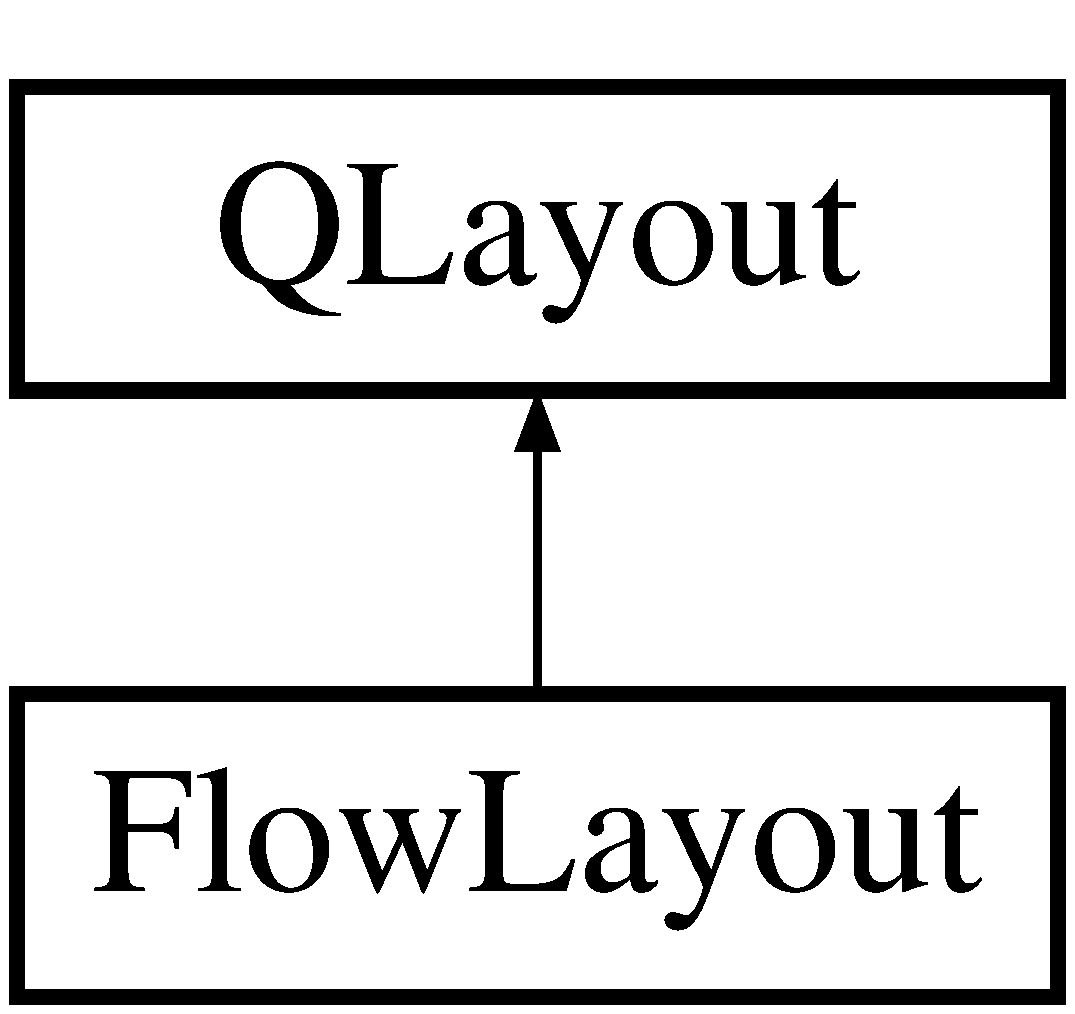
\includegraphics[height=2.000000cm]{classFlowLayout}
\end{center}
\end{figure}
\subsection*{Public Member Functions}
\begin{DoxyCompactItemize}
\item 
\hypertarget{classFlowLayout_afd3623cad3b02592123eb8a4dd01546f}{{\bfseries Flow\+Layout} (Q\+Widget $\ast$parent, int margin=-\/1, int h\+Spacing=-\/1, int v\+Spacing=-\/1)}\label{classFlowLayout_afd3623cad3b02592123eb8a4dd01546f}

\item 
\hypertarget{classFlowLayout_a76357c75560d6bcbee7a4782c852ca07}{{\bfseries Flow\+Layout} (int margin=-\/1, int h\+Spacing=-\/1, int v\+Spacing=-\/1)}\label{classFlowLayout_a76357c75560d6bcbee7a4782c852ca07}

\item 
\hypertarget{classFlowLayout_a6a3f498fdac0145fe38838f31a6336cf}{void {\bfseries add\+Item} (Q\+Layout\+Item $\ast$item)}\label{classFlowLayout_a6a3f498fdac0145fe38838f31a6336cf}

\item 
\hypertarget{classFlowLayout_a214d375a68a3590bf4b947e02eae09a3}{int {\bfseries horizontal\+Spacing} () const }\label{classFlowLayout_a214d375a68a3590bf4b947e02eae09a3}

\item 
\hypertarget{classFlowLayout_a1b15dce81c6bce51290d3b55c35dcd3e}{int {\bfseries vertical\+Spacing} () const }\label{classFlowLayout_a1b15dce81c6bce51290d3b55c35dcd3e}

\item 
\hypertarget{classFlowLayout_a2d2b5413e1e4eff15d23134208812a47}{Qt\+::\+Orientations {\bfseries expanding\+Directions} () const }\label{classFlowLayout_a2d2b5413e1e4eff15d23134208812a47}

\item 
\hypertarget{classFlowLayout_a52203cd7f45648d9aee605b38daf4d87}{bool {\bfseries has\+Height\+For\+Width} () const }\label{classFlowLayout_a52203cd7f45648d9aee605b38daf4d87}

\item 
\hypertarget{classFlowLayout_af976e908e7bd74bd2ceff220739712a9}{int {\bfseries height\+For\+Width} (int) const }\label{classFlowLayout_af976e908e7bd74bd2ceff220739712a9}

\item 
\hypertarget{classFlowLayout_ae0d78c1e30b0bf5346e3ab94b80edeff}{int {\bfseries count} () const }\label{classFlowLayout_ae0d78c1e30b0bf5346e3ab94b80edeff}

\item 
\hypertarget{classFlowLayout_a02d52a0e8ae5cf8672b2bb1537b896f2}{Q\+Layout\+Item $\ast$ {\bfseries item\+At} (int index) const }\label{classFlowLayout_a02d52a0e8ae5cf8672b2bb1537b896f2}

\item 
\hypertarget{classFlowLayout_a6e28537828ad1c477a299df5bc156212}{Q\+Size {\bfseries minimum\+Size} () const }\label{classFlowLayout_a6e28537828ad1c477a299df5bc156212}

\item 
\hypertarget{classFlowLayout_aa33b32ad4916b86b062d427860952d1e}{void {\bfseries set\+Geometry} (const Q\+Rect \&rect)}\label{classFlowLayout_aa33b32ad4916b86b062d427860952d1e}

\item 
\hypertarget{classFlowLayout_a7d52617e64c908d68dc1c75fbb549325}{Q\+Size {\bfseries size\+Hint} () const }\label{classFlowLayout_a7d52617e64c908d68dc1c75fbb549325}

\item 
\hypertarget{classFlowLayout_a55dad3061f24ea01069d6496e55d4aab}{Q\+Layout\+Item $\ast$ {\bfseries take\+At} (int index)}\label{classFlowLayout_a55dad3061f24ea01069d6496e55d4aab}

\end{DoxyCompactItemize}


The documentation for this class was generated from the following files\+:\begin{DoxyCompactItemize}
\item 
view/flowlayout.\+h\item 
view/flowlayout.\+cpp\end{DoxyCompactItemize}

\hypertarget{classFormation}{\section{Formation Class Reference}
\label{classFormation}\index{Formation@{Formation}}
}
Inheritance diagram for Formation\+:\begin{figure}[H]
\begin{center}
\leavevmode
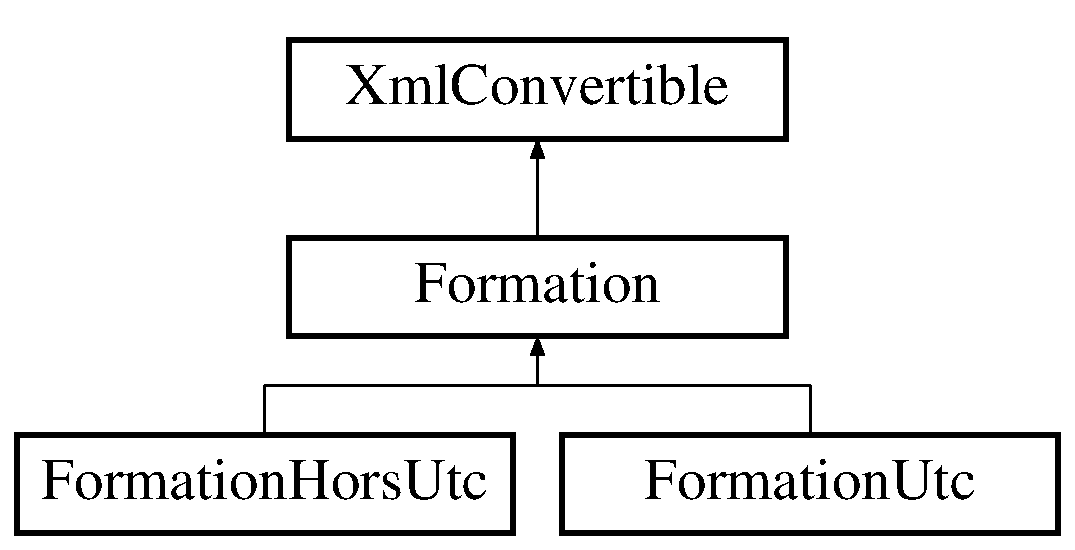
\includegraphics[height=3.000000cm]{classFormation}
\end{center}
\end{figure}
\subsection*{Public Member Functions}
\begin{DoxyCompactItemize}
\item 
\hypertarget{classFormation_ae2554a8a085697bffb5691e9a3eba694}{unsigned int {\bfseries id} () const }\label{classFormation_ae2554a8a085697bffb5691e9a3eba694}

\item 
\hypertarget{classFormation_a94ea9bc0973149c6db430361b0c04367}{unsigned int {\bfseries credits} () const }\label{classFormation_a94ea9bc0973149c6db430361b0c04367}

\item 
\hypertarget{classFormation_aa54c9b0dbe6eec3df39f3c87b8efc4a5}{Q\+String {\bfseries nom} () const }\label{classFormation_aa54c9b0dbe6eec3df39f3c87b8efc4a5}

\item 
\hypertarget{classFormation_a6822ab119dd1cec435dce264d2a07f4b}{void {\bfseries nom} (const Q\+String \&n)}\label{classFormation_a6822ab119dd1cec435dce264d2a07f4b}

\item 
\hypertarget{classFormation_a4c5665c37f7fdaa8421768f9c95aa8c5}{virtual void \hyperlink{classFormation_a4c5665c37f7fdaa8421768f9c95aa8c5}{from\+Xml} (const Q\+Dom\+Node \&noeud)=0}\label{classFormation_a4c5665c37f7fdaa8421768f9c95aa8c5}

\begin{DoxyCompactList}\small\item\em Définit l'objet à partir d'un élément X\+M\+L. \end{DoxyCompactList}\item 
virtual Q\+Dom\+Element \hyperlink{classFormation_aea1a12114f435bba6a32a0a32ca32e47}{to\+Xml} () const =0
\begin{DoxyCompactList}\small\item\em Convertit l'objet au format X\+M\+L. \end{DoxyCompactList}\end{DoxyCompactItemize}


\subsection{Member Function Documentation}
\hypertarget{classFormation_aea1a12114f435bba6a32a0a32ca32e47}{\index{Formation@{Formation}!to\+Xml@{to\+Xml}}
\index{to\+Xml@{to\+Xml}!Formation@{Formation}}
\subsubsection[{to\+Xml}]{\setlength{\rightskip}{0pt plus 5cm}virtual Q\+Dom\+Element Formation\+::to\+Xml (
\begin{DoxyParamCaption}
{}
\end{DoxyParamCaption}
) const\hspace{0.3cm}{\ttfamily [pure virtual]}}}\label{classFormation_aea1a12114f435bba6a32a0a32ca32e47}


Convertit l'objet au format X\+M\+L. 

\begin{DoxyReturn}{Returns}
L'élément X\+M\+L correspondant 
\end{DoxyReturn}


Implements \hyperlink{classXmlConvertible_a188430d1503cf6db7223374306577c2c}{Xml\+Convertible}.



Implemented in \hyperlink{classFormationUtc_a8dcda30820484cd00e82ad53a1b313f9}{Formation\+Utc}, and \hyperlink{classFormationHorsUtc_ab7f0cb9fcecf0423b257d1011e7d8623}{Formation\+Hors\+Utc}.



The documentation for this class was generated from the following files\+:\begin{DoxyCompactItemize}
\item 
model/formation.\+h\item 
model/formation.\+cpp\end{DoxyCompactItemize}

\hypertarget{classFormationController}{\section{Formation\+Controller Class Reference}
\label{classFormationController}\index{Formation\+Controller@{Formation\+Controller}}
}
Inheritance diagram for Formation\+Controller\+:\begin{figure}[H]
\begin{center}
\leavevmode
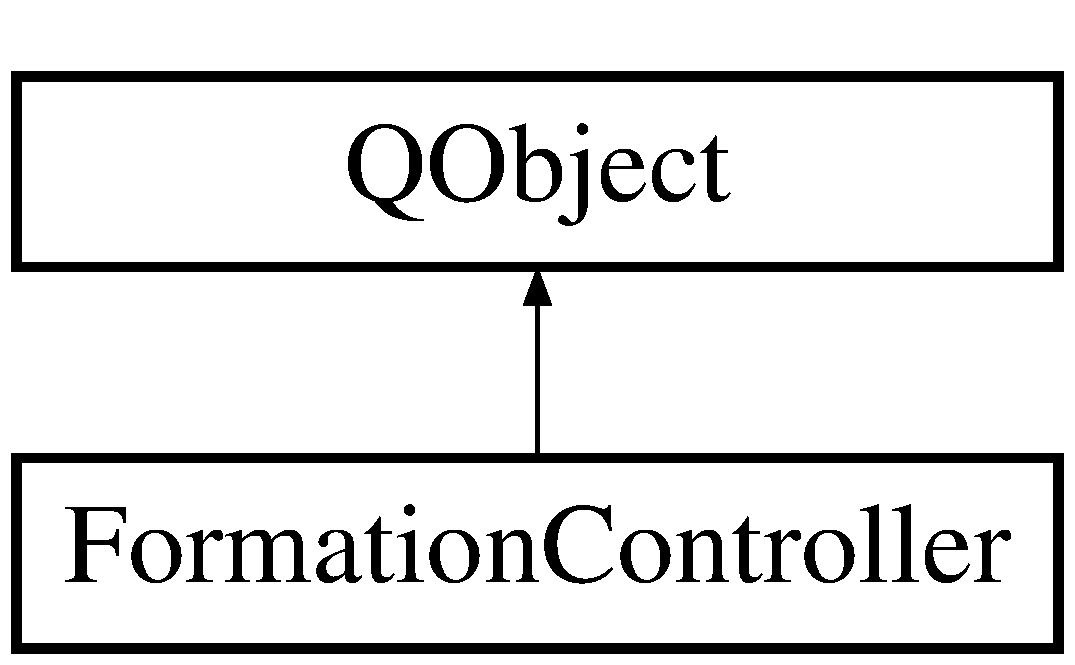
\includegraphics[height=2.000000cm]{classFormationController}
\end{center}
\end{figure}
\subsection*{Public Slots}
\begin{DoxyCompactItemize}
\item 
\hypertarget{classFormationController_a6f209a01ee733426791619c2e17339be}{void {\bfseries edit\+Event} (const Q\+String name, const int credits)}\label{classFormationController_a6f209a01ee733426791619c2e17339be}

\item 
\hypertarget{classFormationController_a77df1d85adb3b9cd5d9baeaee858d87e}{void {\bfseries remove} ()}\label{classFormationController_a77df1d85adb3b9cd5d9baeaee858d87e}

\end{DoxyCompactItemize}
\subsection*{Signals}
\begin{DoxyCompactItemize}
\item 
\hypertarget{classFormationController_a409df906810b5cda8e2d21f0da29b967}{void {\bfseries removed} (\hyperlink{classFormationHorsUtc}{Formation\+Hors\+Utc} $\ast$formation)}\label{classFormationController_a409df906810b5cda8e2d21f0da29b967}

\item 
\hypertarget{classFormationController_aa3391fadf4675a73fcef4ea1fc1353d2}{void {\bfseries \+\_\+removed} ()}\label{classFormationController_aa3391fadf4675a73fcef4ea1fc1353d2}

\end{DoxyCompactItemize}
\subsection*{Public Member Functions}
\begin{DoxyCompactItemize}
\item 
\hypertarget{classFormationController_a0503e366066246aebad060de9dc02c77}{{\bfseries Formation\+Controller} (\hyperlink{classFormationHorsUtc}{Formation\+Hors\+Utc} $\ast$formation, \hyperlink{classQFormation}{Q\+Formation} $\ast$q\+Formation, Q\+Object $\ast$parent=0)}\label{classFormationController_a0503e366066246aebad060de9dc02c77}

\end{DoxyCompactItemize}


The documentation for this class was generated from the following files\+:\begin{DoxyCompactItemize}
\item 
controller/formationcontroller.\+h\item 
controller/formationcontroller.\+cpp\end{DoxyCompactItemize}

\hypertarget{classFormationHorsUtc}{\section{Formation\+Hors\+Utc Class Reference}
\label{classFormationHorsUtc}\index{Formation\+Hors\+Utc@{Formation\+Hors\+Utc}}
}
Inheritance diagram for Formation\+Hors\+Utc\+:\begin{figure}[H]
\begin{center}
\leavevmode
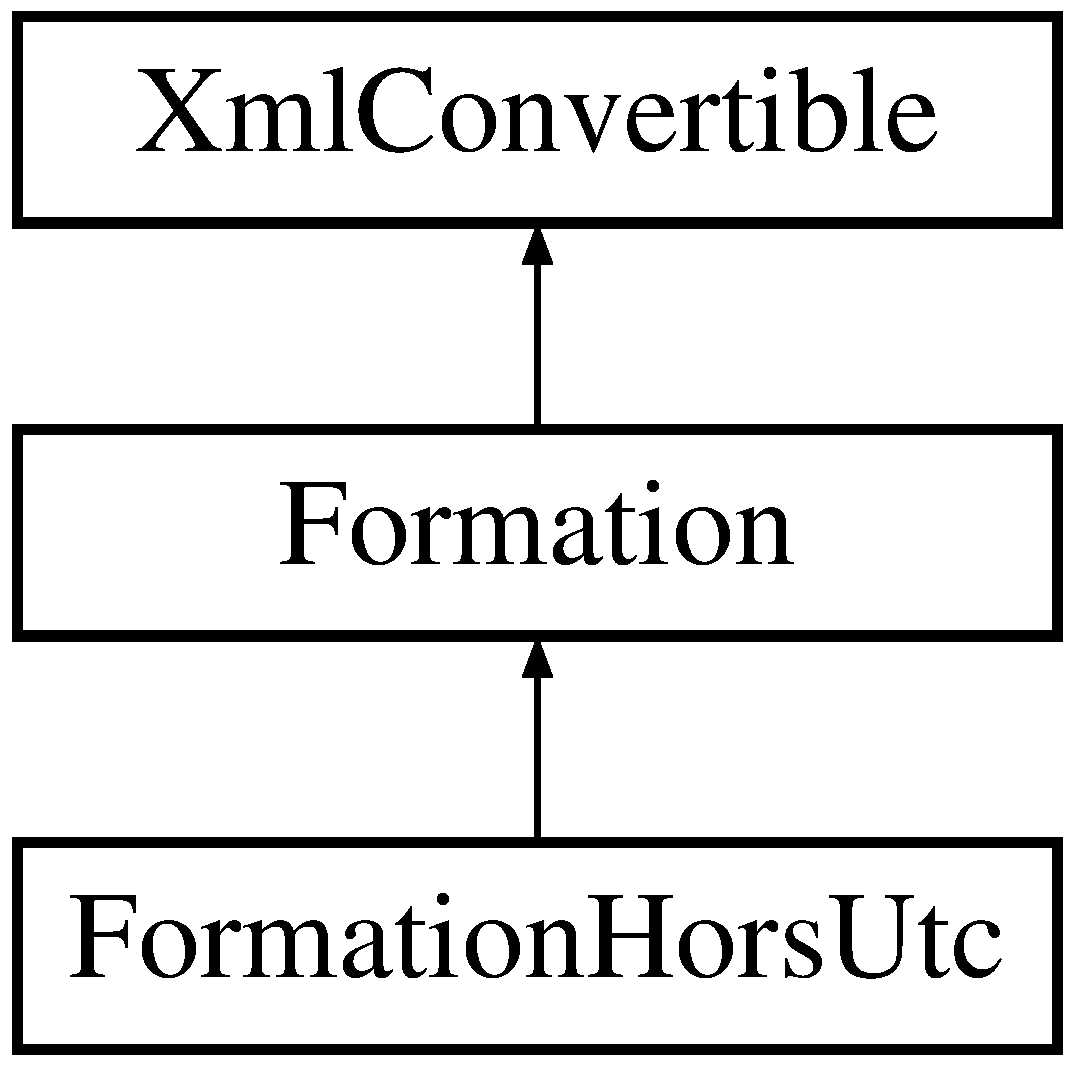
\includegraphics[height=3.000000cm]{classFormationHorsUtc}
\end{center}
\end{figure}
\subsection*{Public Member Functions}
\begin{DoxyCompactItemize}
\item 
\hypertarget{classFormationHorsUtc_a26f00d5dba28d91d3ea440cf3440bbaf}{void \hyperlink{classFormationHorsUtc_a26f00d5dba28d91d3ea440cf3440bbaf}{from\+Xml} (const Q\+Dom\+Node \&noeud)}\label{classFormationHorsUtc_a26f00d5dba28d91d3ea440cf3440bbaf}

\begin{DoxyCompactList}\small\item\em Définit l'objet à partir d'un élément X\+M\+L. \end{DoxyCompactList}\item 
Q\+Dom\+Element \hyperlink{classFormationHorsUtc_ab7f0cb9fcecf0423b257d1011e7d8623}{to\+Xml} () const 
\begin{DoxyCompactList}\small\item\em Convertit l'objet au format X\+M\+L. \end{DoxyCompactList}\item 
\hypertarget{classFormationHorsUtc_a8a62e27ab27a640f099b26eaebc2ebc0}{unsigned int {\bfseries credits} () const }\label{classFormationHorsUtc_a8a62e27ab27a640f099b26eaebc2ebc0}

\item 
\hypertarget{classFormationHorsUtc_ac59e7234fbe648389906940b6f67645f}{Q\+String {\bfseries nom} () const }\label{classFormationHorsUtc_ac59e7234fbe648389906940b6f67645f}

\item 
\hypertarget{classFormationHorsUtc_a7488a55025f57f319a1fab33ad1ea830}{void {\bfseries nom} (const Q\+String \&n)}\label{classFormationHorsUtc_a7488a55025f57f319a1fab33ad1ea830}

\item 
\hypertarget{classFormationHorsUtc_a9e6fba7076ad67ff52fc07579083cdcf}{void {\bfseries credits} (unsigned int c)}\label{classFormationHorsUtc_a9e6fba7076ad67ff52fc07579083cdcf}

\end{DoxyCompactItemize}
\subsection*{Static Public Attributes}
\begin{DoxyCompactItemize}
\item 
\hypertarget{classFormationHorsUtc_acd847f2459d576c1612607a66526e925}{static const Q\+String \hyperlink{classFormationHorsUtc_acd847f2459d576c1612607a66526e925}{X\+M\+L\+\_\+\+N\+O\+D\+E\+\_\+\+N\+A\+M\+E} = \char`\"{}formation-\/hors-\/utc\char`\"{}}\label{classFormationHorsUtc_acd847f2459d576c1612607a66526e925}

\begin{DoxyCompactList}\small\item\em Nom du noeud X\+M\+L correspondant à une formation hors utc. \end{DoxyCompactList}\end{DoxyCompactItemize}


\subsection{Member Function Documentation}
\hypertarget{classFormationHorsUtc_ab7f0cb9fcecf0423b257d1011e7d8623}{\index{Formation\+Hors\+Utc@{Formation\+Hors\+Utc}!to\+Xml@{to\+Xml}}
\index{to\+Xml@{to\+Xml}!Formation\+Hors\+Utc@{Formation\+Hors\+Utc}}
\subsubsection[{to\+Xml}]{\setlength{\rightskip}{0pt plus 5cm}Q\+Dom\+Element Formation\+Hors\+Utc\+::to\+Xml (
\begin{DoxyParamCaption}
{}
\end{DoxyParamCaption}
) const\hspace{0.3cm}{\ttfamily [virtual]}}}\label{classFormationHorsUtc_ab7f0cb9fcecf0423b257d1011e7d8623}


Convertit l'objet au format X\+M\+L. 

\begin{DoxyReturn}{Returns}
L'élément X\+M\+L correspondant 
\end{DoxyReturn}


Implements \hyperlink{classFormation_aea1a12114f435bba6a32a0a32ca32e47}{Formation}.



The documentation for this class was generated from the following files\+:\begin{DoxyCompactItemize}
\item 
model/formation\+Hors\+Utc.\+h\item 
model/formation\+Hors\+Utc.\+cpp\end{DoxyCompactItemize}

\hypertarget{classFormationUtc}{\section{Formation\+Utc Class Reference}
\label{classFormationUtc}\index{Formation\+Utc@{Formation\+Utc}}
}
Inheritance diagram for Formation\+Utc\+:\begin{figure}[H]
\begin{center}
\leavevmode
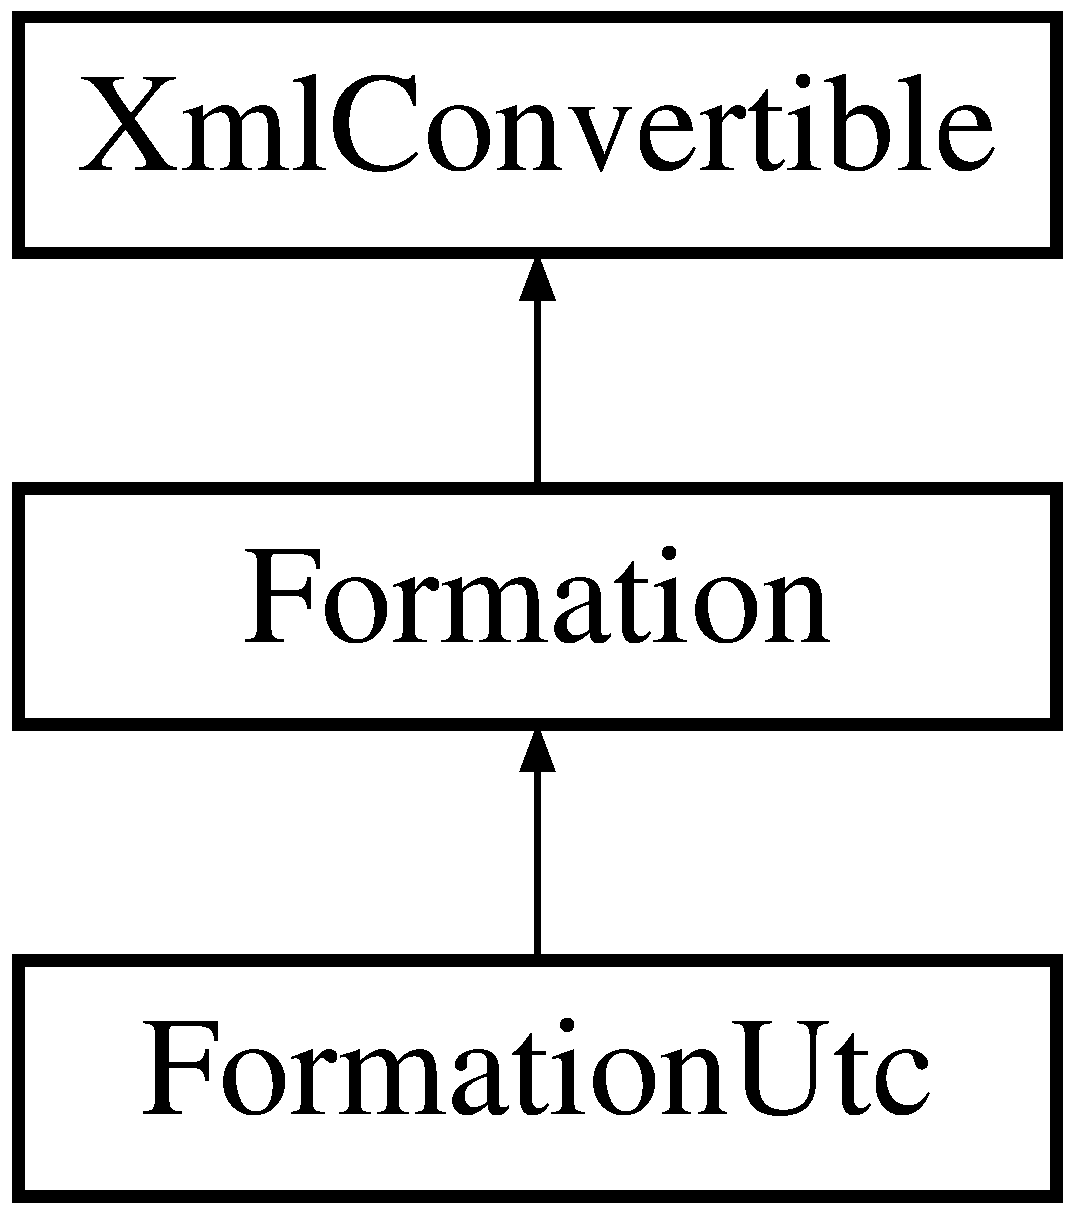
\includegraphics[height=3.000000cm]{classFormationUtc}
\end{center}
\end{figure}
\subsection*{Public Member Functions}
\begin{DoxyCompactItemize}
\item 
void \hyperlink{classFormationUtc_a9922944f1ec47720995c836b1eb7eea7}{ajouter\+Semestre} (\hyperlink{classSemestre}{Semestre} $\ast$s)
\begin{DoxyCompactList}\small\item\em Ajoute un semestre à la formation. \end{DoxyCompactList}\item 
void \hyperlink{classFormationUtc_ac3af0dcb7092a12790d979496c466466}{supprimer\+Semestre} (int id)
\begin{DoxyCompactList}\small\item\em Supprime un semestre de la formation. \end{DoxyCompactList}\item 
\hypertarget{classFormationUtc_a370bec2b5e818d45fd4b447500fb7a57}{void \hyperlink{classFormationUtc_a370bec2b5e818d45fd4b447500fb7a57}{from\+Xml} (const Q\+Dom\+Node \&noeud)}\label{classFormationUtc_a370bec2b5e818d45fd4b447500fb7a57}

\begin{DoxyCompactList}\small\item\em Définit l'objet à partir d'un élément X\+M\+L. \end{DoxyCompactList}\item 
Q\+Dom\+Element \hyperlink{classFormationUtc_a8dcda30820484cd00e82ad53a1b313f9}{to\+Xml} () const 
\begin{DoxyCompactList}\small\item\em Convertit l'objet au format X\+M\+L. \end{DoxyCompactList}\item 
\hypertarget{classFormationUtc_a144b0074f75c3ccdbd02974581758484}{Q\+List$<$ \hyperlink{classSemestre}{Semestre} $\ast$ $>$ {\bfseries semestres} () const }\label{classFormationUtc_a144b0074f75c3ccdbd02974581758484}

\item 
\hypertarget{classFormationUtc_a7f6f00890a69b763544791bf0310d892}{unsigned int {\bfseries id} () const }\label{classFormationUtc_a7f6f00890a69b763544791bf0310d892}

\item 
\hypertarget{classFormationUtc_a5b09b2e9c99fcaa643991acdab2c4117}{unsigned int {\bfseries credits} () const }\label{classFormationUtc_a5b09b2e9c99fcaa643991acdab2c4117}

\item 
\hypertarget{classFormationUtc_a9940a7fae66a24fdff63e862a3b5d0b7}{Q\+String {\bfseries nom} () const }\label{classFormationUtc_a9940a7fae66a24fdff63e862a3b5d0b7}

\item 
\hypertarget{classFormationUtc_ab9be42a9ee817c07d473a08e0684c453}{void {\bfseries nom} (const Q\+String \&n)}\label{classFormationUtc_ab9be42a9ee817c07d473a08e0684c453}

\item 
bool \hyperlink{classFormationUtc_a188a5be3b7561d558cdafde750f302b5}{uv\+Deja\+Validee} (const Q\+String \&tag, \hyperlink{classUVEtudiant}{U\+V\+Etudiant} $\ast$uv=0) const 
\end{DoxyCompactItemize}
\subsection*{Static Public Attributes}
\begin{DoxyCompactItemize}
\item 
\hypertarget{classFormationUtc_ab4939306e72edabdc484f3c1b208507e}{static const Q\+String \hyperlink{classFormationUtc_ab4939306e72edabdc484f3c1b208507e}{X\+M\+L\+\_\+\+N\+O\+D\+E\+\_\+\+N\+A\+M\+E} = \char`\"{}formation-\/utc\char`\"{}}\label{classFormationUtc_ab4939306e72edabdc484f3c1b208507e}

\begin{DoxyCompactList}\small\item\em Nom du noeud X\+M\+L correspondant à une formation hors utc. \end{DoxyCompactList}\end{DoxyCompactItemize}


\subsection{Member Function Documentation}
\hypertarget{classFormationUtc_a9922944f1ec47720995c836b1eb7eea7}{\index{Formation\+Utc@{Formation\+Utc}!ajouter\+Semestre@{ajouter\+Semestre}}
\index{ajouter\+Semestre@{ajouter\+Semestre}!Formation\+Utc@{Formation\+Utc}}
\subsubsection[{ajouter\+Semestre}]{\setlength{\rightskip}{0pt plus 5cm}void Formation\+Utc\+::ajouter\+Semestre (
\begin{DoxyParamCaption}
\item[{{\bf Semestre} $\ast$}]{s}
\end{DoxyParamCaption}
)}}\label{classFormationUtc_a9922944f1ec47720995c836b1eb7eea7}


Ajoute un semestre à la formation. 


\begin{DoxyParams}{Parameters}
{\em s} & Le semestre à ajouter \\
\hline
\end{DoxyParams}
\hypertarget{classFormationUtc_ac3af0dcb7092a12790d979496c466466}{\index{Formation\+Utc@{Formation\+Utc}!supprimer\+Semestre@{supprimer\+Semestre}}
\index{supprimer\+Semestre@{supprimer\+Semestre}!Formation\+Utc@{Formation\+Utc}}
\subsubsection[{supprimer\+Semestre}]{\setlength{\rightskip}{0pt plus 5cm}void Formation\+Utc\+::supprimer\+Semestre (
\begin{DoxyParamCaption}
\item[{int}]{id}
\end{DoxyParamCaption}
)}}\label{classFormationUtc_ac3af0dcb7092a12790d979496c466466}


Supprime un semestre de la formation. 


\begin{DoxyParams}{Parameters}
{\em id} & L'identifiant du semestre à supprimer \\
\hline
\end{DoxyParams}
\hypertarget{classFormationUtc_a8dcda30820484cd00e82ad53a1b313f9}{\index{Formation\+Utc@{Formation\+Utc}!to\+Xml@{to\+Xml}}
\index{to\+Xml@{to\+Xml}!Formation\+Utc@{Formation\+Utc}}
\subsubsection[{to\+Xml}]{\setlength{\rightskip}{0pt plus 5cm}Q\+Dom\+Element Formation\+Utc\+::to\+Xml (
\begin{DoxyParamCaption}
{}
\end{DoxyParamCaption}
) const\hspace{0.3cm}{\ttfamily [virtual]}}}\label{classFormationUtc_a8dcda30820484cd00e82ad53a1b313f9}


Convertit l'objet au format X\+M\+L. 

\begin{DoxyReturn}{Returns}
L'élément X\+M\+L correspondant 
\end{DoxyReturn}


Implements \hyperlink{classFormation_aea1a12114f435bba6a32a0a32ca32e47}{Formation}.

\hypertarget{classFormationUtc_a188a5be3b7561d558cdafde750f302b5}{\index{Formation\+Utc@{Formation\+Utc}!uv\+Deja\+Validee@{uv\+Deja\+Validee}}
\index{uv\+Deja\+Validee@{uv\+Deja\+Validee}!Formation\+Utc@{Formation\+Utc}}
\subsubsection[{uv\+Deja\+Validee}]{\setlength{\rightskip}{0pt plus 5cm}bool Formation\+Utc\+::uv\+Deja\+Validee (
\begin{DoxyParamCaption}
\item[{const Q\+String \&}]{tag, }
\item[{{\bf U\+V\+Etudiant} $\ast$}]{uv = {\ttfamily 0}}
\end{DoxyParamCaption}
) const}}\label{classFormationUtc_a188a5be3b7561d558cdafde750f302b5}

\begin{DoxyParams}{Parameters}
{\em tag} & Le tag de l'uv \\
\hline
{\em uv} & L'uv contenant la note de l'étudiant si l'uv a été validée\\
\hline
\end{DoxyParams}
\begin{DoxyReturn}{Returns}
Vrai si l'uv a été validée par l'étudiant, faux sinon 
\end{DoxyReturn}


The documentation for this class was generated from the following files\+:\begin{DoxyCompactItemize}
\item 
model/formation\+Utc.\+h\item 
model/formation\+Utc.\+cpp\end{DoxyCompactItemize}

\hypertarget{classMainWindow}{\section{Main\+Window Class Reference}
\label{classMainWindow}\index{Main\+Window@{Main\+Window}}
}
Inheritance diagram for Main\+Window\+:\begin{figure}[H]
\begin{center}
\leavevmode
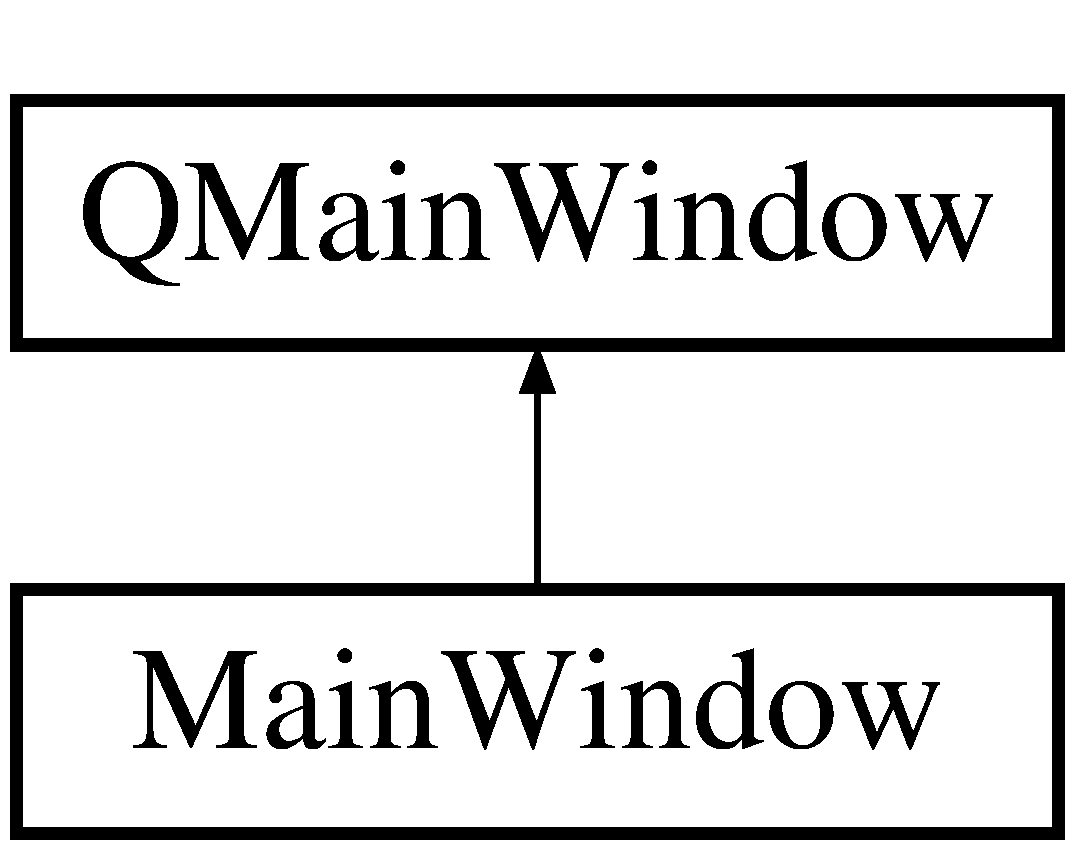
\includegraphics[height=2.000000cm]{classMainWindow}
\end{center}
\end{figure}
\subsection*{Public Slots}
\begin{DoxyCompactItemize}
\item 
\hypertarget{classMainWindow_ae57c5976e1e8afb836fc0668aaaa000c}{void {\bfseries button\+Add\+Formation\+Clicked} ()}\label{classMainWindow_ae57c5976e1e8afb836fc0668aaaa000c}

\item 
\hypertarget{classMainWindow_ac92e784d08c3797023da714057db1cfc}{void {\bfseries button\+Add\+Semestre\+Clicked} ()}\label{classMainWindow_ac92e784d08c3797023da714057db1cfc}

\item 
\hypertarget{classMainWindow_a5966da1b123ebab9fa12804a650148db}{void {\bfseries edit\+Name\+Changed} (const Q\+String \&text)}\label{classMainWindow_a5966da1b123ebab9fa12804a650148db}

\item 
\hypertarget{classMainWindow_a0d4a0102449a45525b9877b93ff5abb4}{void {\bfseries edit\+Surname\+Changed} (const Q\+String \&text)}\label{classMainWindow_a0d4a0102449a45525b9877b93ff5abb4}

\end{DoxyCompactItemize}
\subsection*{Signals}
\begin{DoxyCompactItemize}
\item 
\hypertarget{classMainWindow_a10491cf43441856bb6909de69b5bedcb}{void {\bfseries add\+Formation\+Clicked} ()}\label{classMainWindow_a10491cf43441856bb6909de69b5bedcb}

\item 
\hypertarget{classMainWindow_a6eab6e752afad90ad02c97522cbc0db9}{void {\bfseries add\+Semestre\+Clicked} ()}\label{classMainWindow_a6eab6e752afad90ad02c97522cbc0db9}

\item 
\hypertarget{classMainWindow_aef78295e40864463c856aeb47f00ff83}{void {\bfseries name\+Changed} (const Q\+String \&name, const Q\+String \&surname)}\label{classMainWindow_aef78295e40864463c856aeb47f00ff83}

\end{DoxyCompactItemize}
\subsection*{Public Member Functions}
\begin{DoxyCompactItemize}
\item 
\hypertarget{classMainWindow_a8b244be8b7b7db1b08de2a2acb9409db}{{\bfseries Main\+Window} (Q\+Widget $\ast$parent=0)}\label{classMainWindow_a8b244be8b7b7db1b08de2a2acb9409db}

\item 
\hypertarget{classMainWindow_a2cc7c0de101c3d1e71d0c820caaa090c}{void {\bfseries set\+Name} (const Q\+String \&name, const Q\+String \&surname)}\label{classMainWindow_a2cc7c0de101c3d1e71d0c820caaa090c}

\item 
\hypertarget{classMainWindow_a0a7af10fa2c844b50c01c48e165d8791}{void {\bfseries add\+Formation} (\hyperlink{classQFormation}{Q\+Formation} $\ast$formation)}\label{classMainWindow_a0a7af10fa2c844b50c01c48e165d8791}

\item 
\hypertarget{classMainWindow_a8806edf1fc9c44ae0c05752f75cd03b9}{void {\bfseries add\+Semestre} (\hyperlink{classQSemestre}{Q\+Semestre} $\ast$semestre)}\label{classMainWindow_a8806edf1fc9c44ae0c05752f75cd03b9}

\end{DoxyCompactItemize}


The documentation for this class was generated from the following files\+:\begin{DoxyCompactItemize}
\item 
view/mainwindow.\+h\item 
view/mainwindow.\+cpp\end{DoxyCompactItemize}

\hypertarget{classMainWindowController}{\section{Main\+Window\+Controller Class Reference}
\label{classMainWindowController}\index{Main\+Window\+Controller@{Main\+Window\+Controller}}
}
Inheritance diagram for Main\+Window\+Controller\+:\begin{figure}[H]
\begin{center}
\leavevmode
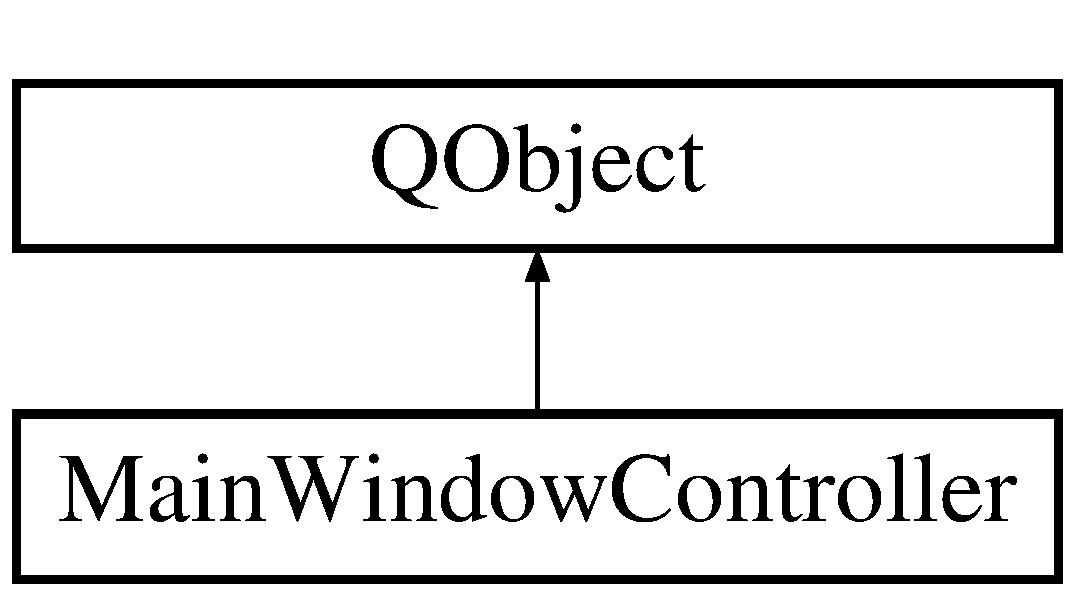
\includegraphics[height=2.000000cm]{classMainWindowController}
\end{center}
\end{figure}
\subsection*{Public Slots}
\begin{DoxyCompactItemize}
\item 
\hypertarget{classMainWindowController_abc59d49d0b3a28567709eea4f6c235b0}{void {\bfseries user\+Select} (const int index)}\label{classMainWindowController_abc59d49d0b3a28567709eea4f6c235b0}

\item 
\hypertarget{classMainWindowController_af706e644d430a17b28751b4b68d7e098}{void {\bfseries user\+Select\+Rejected} ()}\label{classMainWindowController_af706e644d430a17b28751b4b68d7e098}

\item 
\hypertarget{classMainWindowController_a8f8eb0a351a447ef76289140cfebbec2}{void {\bfseries name\+Changed} (const Q\+String \&name, const Q\+String \&surname)}\label{classMainWindowController_a8f8eb0a351a447ef76289140cfebbec2}

\item 
\hypertarget{classMainWindowController_a839f58b4aa76126f41e79e58d83814a7}{void {\bfseries add\+Formation} ()}\label{classMainWindowController_a839f58b4aa76126f41e79e58d83814a7}

\item 
\hypertarget{classMainWindowController_a5e87d3e09120071039146bdc20939d03}{void {\bfseries add\+Semestre} ()}\label{classMainWindowController_a5e87d3e09120071039146bdc20939d03}

\item 
\hypertarget{classMainWindowController_af447b7baea272507e216431c821b3e9c}{void {\bfseries remove\+Formation} (\hyperlink{classFormationHorsUtc}{Formation\+Hors\+Utc} $\ast$formation)}\label{classMainWindowController_af447b7baea272507e216431c821b3e9c}

\item 
\hypertarget{classMainWindowController_afa1bdec4bbb04d6413574603e08fffb9}{void {\bfseries remove\+Semestre} (\hyperlink{classSemestre}{Semestre} $\ast$semestre)}\label{classMainWindowController_afa1bdec4bbb04d6413574603e08fffb9}

\item 
\hypertarget{classMainWindowController_a656ad663043162f57664135f87f3524b}{void {\bfseries exiting} ()}\label{classMainWindowController_a656ad663043162f57664135f87f3524b}

\end{DoxyCompactItemize}
\subsection*{Public Member Functions}
\begin{DoxyCompactItemize}
\item 
\hypertarget{classMainWindowController_a123ba7b98ffb51986b1d42e552c21762}{{\bfseries Main\+Window\+Controller} (Q\+Application \&a)}\label{classMainWindowController_a123ba7b98ffb51986b1d42e552c21762}

\end{DoxyCompactItemize}


The documentation for this class was generated from the following files\+:\begin{DoxyCompactItemize}
\item 
controller/mainwindowcontroller.\+h\item 
controller/mainwindowcontroller.\+cpp\end{DoxyCompactItemize}

\hypertarget{classQFiltreBranche}{\section{Q\+Filtre\+Branche Class Reference}
\label{classQFiltreBranche}\index{Q\+Filtre\+Branche@{Q\+Filtre\+Branche}}
}
Inheritance diagram for Q\+Filtre\+Branche\+:\begin{figure}[H]
\begin{center}
\leavevmode
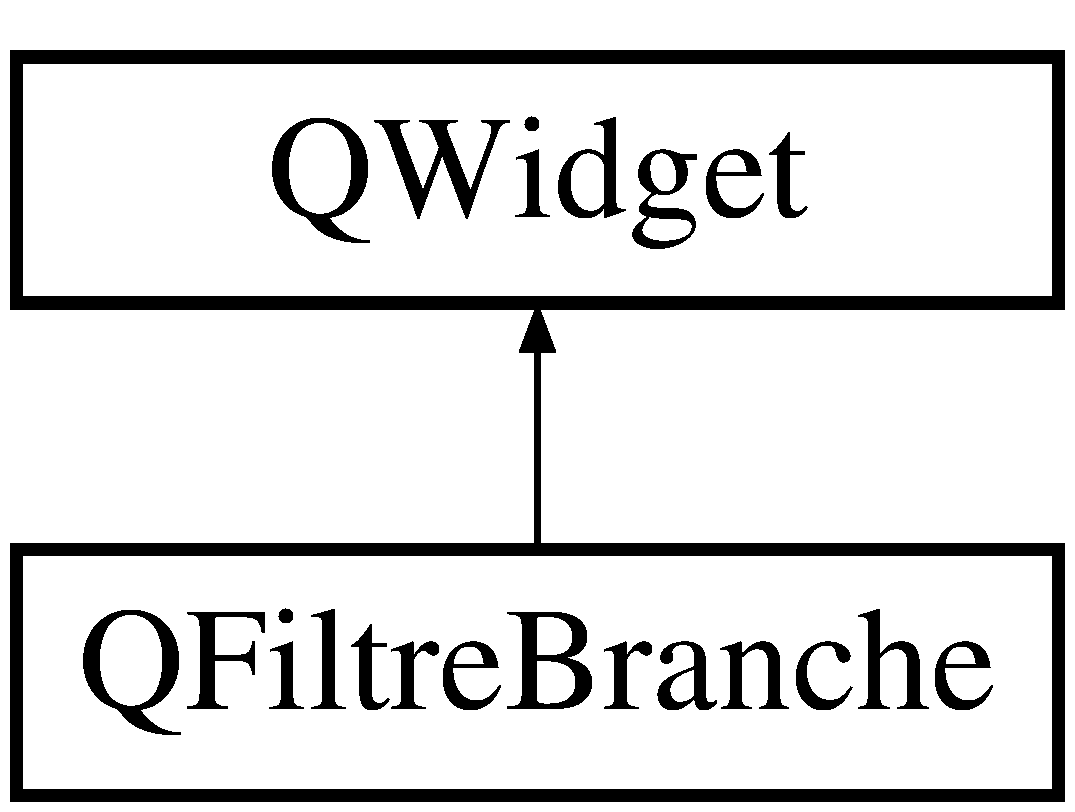
\includegraphics[height=2.000000cm]{classQFiltreBranche}
\end{center}
\end{figure}
\subsection*{Public Slots}
\begin{DoxyCompactItemize}
\item 
\hypertarget{classQFiltreBranche_a26b7d1d502beded039d21490a7767c21}{void {\bfseries all\+Toggled} (bool v)}\label{classQFiltreBranche_a26b7d1d502beded039d21490a7767c21}

\item 
\hypertarget{classQFiltreBranche_a03494ad495b4f96475b9ce0241ce8ecc}{void {\bfseries check\+Box} (bool v)}\label{classQFiltreBranche_a03494ad495b4f96475b9ce0241ce8ecc}

\end{DoxyCompactItemize}
\subsection*{Signals}
\begin{DoxyCompactItemize}
\item 
\hypertarget{classQFiltreBranche_aab3bc72e3317c77916c15039368c2249}{void {\bfseries filter\+Changed} (Q\+String\+List)}\label{classQFiltreBranche_aab3bc72e3317c77916c15039368c2249}

\end{DoxyCompactItemize}
\subsection*{Public Member Functions}
\begin{DoxyCompactItemize}
\item 
\hypertarget{classQFiltreBranche_a9d4428348ef3056d052a93681d489c6d}{{\bfseries Q\+Filtre\+Branche} (Q\+Widget $\ast$parent=0)}\label{classQFiltreBranche_a9d4428348ef3056d052a93681d489c6d}

\item 
\hypertarget{classQFiltreBranche_a1c845f09ab958e4d138c0e856f2569dd}{void {\bfseries add\+Branches} (Q\+String\+List liste\+Branches)}\label{classQFiltreBranche_a1c845f09ab958e4d138c0e856f2569dd}

\end{DoxyCompactItemize}


The documentation for this class was generated from the following files\+:\begin{DoxyCompactItemize}
\item 
view/qfiltrebranche.\+h\item 
view/qfiltrebranche.\+cpp\end{DoxyCompactItemize}

\hypertarget{classQFormation}{\section{Q\+Formation Class Reference}
\label{classQFormation}\index{Q\+Formation@{Q\+Formation}}
}
Inheritance diagram for Q\+Formation\+:\begin{figure}[H]
\begin{center}
\leavevmode
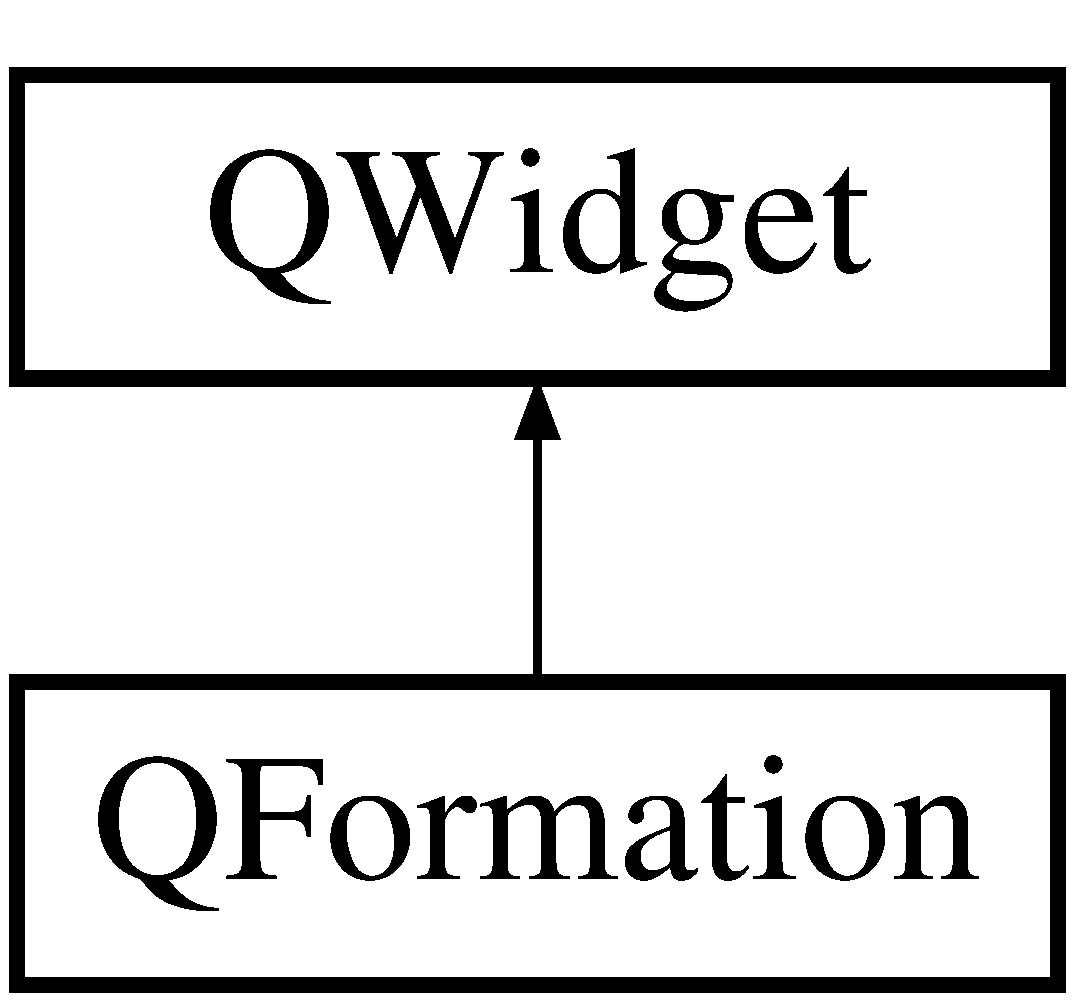
\includegraphics[height=2.000000cm]{classQFormation}
\end{center}
\end{figure}
\subsection*{Public Slots}
\begin{DoxyCompactItemize}
\item 
\hypertarget{classQFormation_a370fb5cd5d5867a27c678847d3913ad9}{void {\bfseries button\+Remove\+Clicked} ()}\label{classQFormation_a370fb5cd5d5867a27c678847d3913ad9}

\item 
\hypertarget{classQFormation_ac2be6e760b1049ec80bec61ecf1ada63}{void {\bfseries edited\+Name} (Q\+String name)}\label{classQFormation_ac2be6e760b1049ec80bec61ecf1ada63}

\item 
\hypertarget{classQFormation_ae7e30ca7fad2caabda0e092e9344e4f9}{void {\bfseries edited\+Credits} (int credits)}\label{classQFormation_ae7e30ca7fad2caabda0e092e9344e4f9}

\end{DoxyCompactItemize}
\subsection*{Signals}
\begin{DoxyCompactItemize}
\item 
\hypertarget{classQFormation_a79fbef8124cc0a48c01cac1d38b6f3e7}{void {\bfseries remove} ()}\label{classQFormation_a79fbef8124cc0a48c01cac1d38b6f3e7}

\item 
\hypertarget{classQFormation_a8c623f0e0278e69e42947b9af6913f14}{void {\bfseries edited} (const Q\+String name, const int credits)}\label{classQFormation_a8c623f0e0278e69e42947b9af6913f14}

\end{DoxyCompactItemize}
\subsection*{Public Member Functions}
\begin{DoxyCompactItemize}
\item 
\hypertarget{classQFormation_aada4a1b24fc353a2b320d04c6269b41b}{{\bfseries Q\+Formation} (Q\+Widget $\ast$parent=0)}\label{classQFormation_aada4a1b24fc353a2b320d04c6269b41b}

\item 
\hypertarget{classQFormation_ae7162d1fe4740f300d314fdbca9d1e64}{void {\bfseries edit} (Q\+String name, int credits)}\label{classQFormation_ae7162d1fe4740f300d314fdbca9d1e64}

\end{DoxyCompactItemize}


The documentation for this class was generated from the following files\+:\begin{DoxyCompactItemize}
\item 
view/qformation.\+h\item 
view/qformation.\+cpp\end{DoxyCompactItemize}

\hypertarget{classQSemestre}{\section{Q\+Semestre Class Reference}
\label{classQSemestre}\index{Q\+Semestre@{Q\+Semestre}}
}
Inheritance diagram for Q\+Semestre\+:\begin{figure}[H]
\begin{center}
\leavevmode
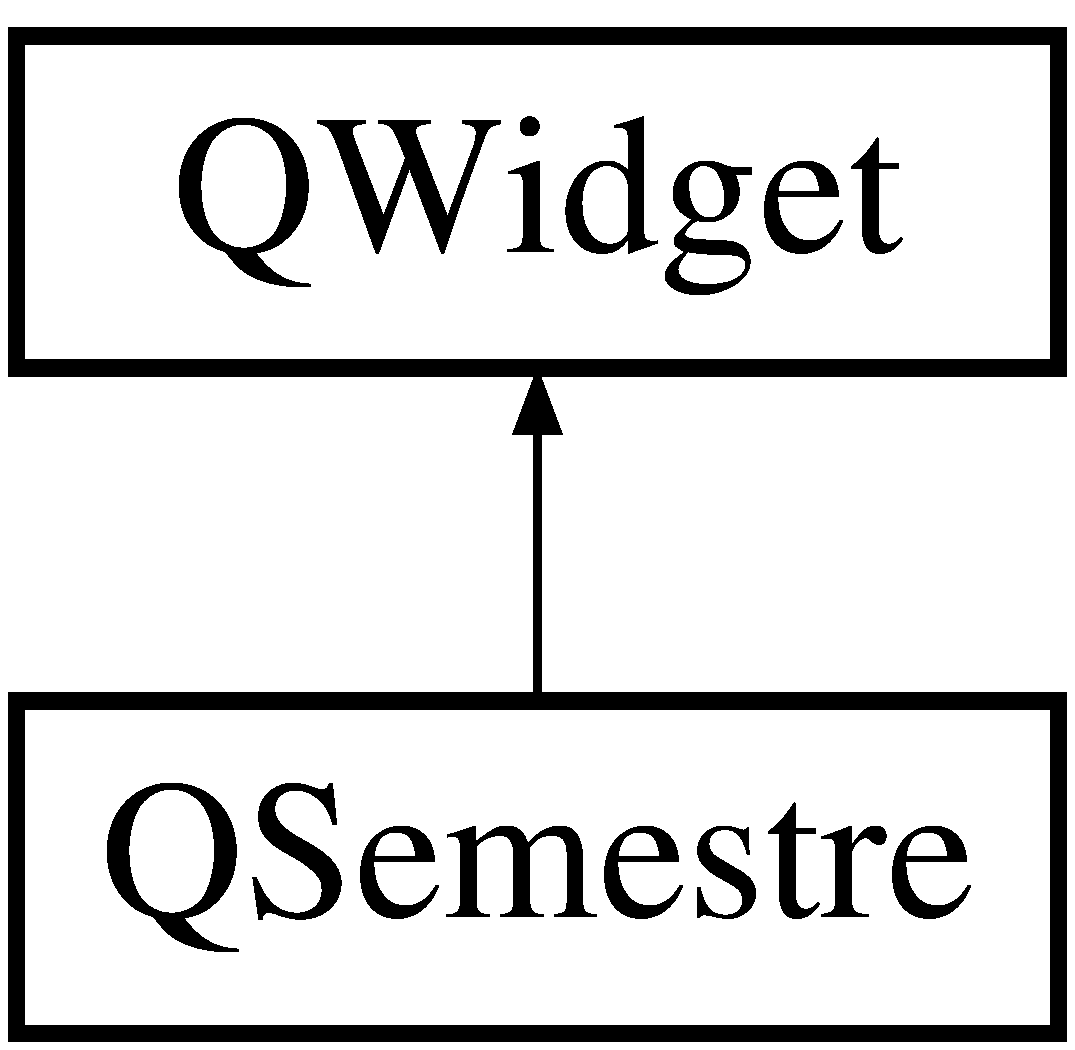
\includegraphics[height=2.000000cm]{classQSemestre}
\end{center}
\end{figure}
\subsection*{Public Slots}
\begin{DoxyCompactItemize}
\item 
\hypertarget{classQSemestre_ac09eff6f409966a2b4bb8b4a6a2d5507}{void {\bfseries button\+Edit\+Clicked} ()}\label{classQSemestre_ac09eff6f409966a2b4bb8b4a6a2d5507}

\item 
\hypertarget{classQSemestre_a864686d70b98929ddbc5d1c8390c1bdb}{void {\bfseries button\+Delete\+Clicked} ()}\label{classQSemestre_a864686d70b98929ddbc5d1c8390c1bdb}

\end{DoxyCompactItemize}
\subsection*{Signals}
\begin{DoxyCompactItemize}
\item 
\hypertarget{classQSemestre_a7ec51eca19ce97c665c2b288a756f3a0}{void {\bfseries edit\+Clicked} ()}\label{classQSemestre_a7ec51eca19ce97c665c2b288a756f3a0}

\item 
\hypertarget{classQSemestre_af32fd11f9440770dec1ac5deb7d62e10}{void {\bfseries delete\+Clicked} ()}\label{classQSemestre_af32fd11f9440770dec1ac5deb7d62e10}

\end{DoxyCompactItemize}
\subsection*{Public Member Functions}
\begin{DoxyCompactItemize}
\item 
\hypertarget{classQSemestre_a1de8cbdf9565a02c82d42249b3d85385}{{\bfseries Q\+Semestre} (Q\+Widget $\ast$parent=0)}\label{classQSemestre_a1de8cbdf9565a02c82d42249b3d85385}

\item 
\hypertarget{classQSemestre_a8cf64a11af7dffe04cb5f94ad0f1106e}{void {\bfseries set\+Date} (Q\+String d)}\label{classQSemestre_a8cf64a11af7dffe04cb5f94ad0f1106e}

\item 
\hypertarget{classQSemestre_ac2b21d3e479163792c19c80b26593024}{Q\+Abstract\+Item\+Model $\ast$ {\bfseries swap\+Model} (Q\+Abstract\+Item\+Model $\ast$model)}\label{classQSemestre_ac2b21d3e479163792c19c80b26593024}

\end{DoxyCompactItemize}


The documentation for this class was generated from the following files\+:\begin{DoxyCompactItemize}
\item 
view/qsemestre.\+h\item 
view/qsemestre.\+cpp\end{DoxyCompactItemize}

\hypertarget{classQSemestreDialog}{\section{Q\+Semestre\+Dialog Class Reference}
\label{classQSemestreDialog}\index{Q\+Semestre\+Dialog@{Q\+Semestre\+Dialog}}
}
Inheritance diagram for Q\+Semestre\+Dialog\+:\begin{figure}[H]
\begin{center}
\leavevmode
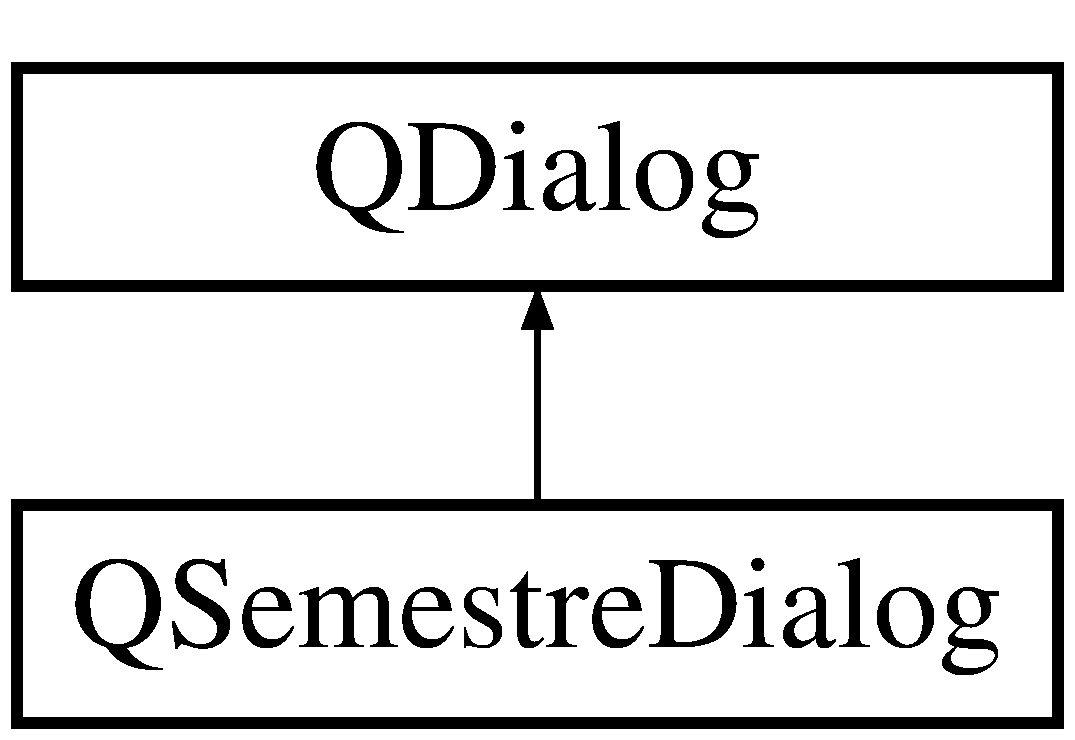
\includegraphics[height=2.000000cm]{classQSemestreDialog}
\end{center}
\end{figure}
\subsection*{Public Slots}
\begin{DoxyCompactItemize}
\item 
\hypertarget{classQSemestreDialog_adaa121f00dc58b7fab93db3bad686b91}{void {\bfseries saison\+Clicked} ()}\label{classQSemestreDialog_adaa121f00dc58b7fab93db3bad686b91}

\item 
\hypertarget{classQSemestreDialog_a6a4c1e728db14181a9d105f423bc2f9e}{void {\bfseries spin\+Year\+Changed} (int year)}\label{classQSemestreDialog_a6a4c1e728db14181a9d105f423bc2f9e}

\end{DoxyCompactItemize}
\subsection*{Signals}
\begin{DoxyCompactItemize}
\item 
\hypertarget{classQSemestreDialog_aa65d57ae77e7e30eb21efdf9e62a26af}{void {\bfseries saison\+Changed} ()}\label{classQSemestreDialog_aa65d57ae77e7e30eb21efdf9e62a26af}

\item 
\hypertarget{classQSemestreDialog_a7d86c777e09a67ffc48b98366be8d2b1}{void {\bfseries year\+Changed} (int year)}\label{classQSemestreDialog_a7d86c777e09a67ffc48b98366be8d2b1}

\end{DoxyCompactItemize}
\subsection*{Public Member Functions}
\begin{DoxyCompactItemize}
\item 
\hypertarget{classQSemestreDialog_afcea6ad11ac7bd74ab93733034932610}{{\bfseries Q\+Semestre\+Dialog} (Q\+Widget $\ast$parent=0)}\label{classQSemestreDialog_afcea6ad11ac7bd74ab93733034932610}

\item 
\hypertarget{classQSemestreDialog_a3e0d0c4df63f736ca56129109d5fcfc9}{void {\bfseries set\+Saison} (Q\+String s)}\label{classQSemestreDialog_a3e0d0c4df63f736ca56129109d5fcfc9}

\item 
\hypertarget{classQSemestreDialog_a84d22926ad386a89cdfff95881616837}{void {\bfseries set\+Year} (int year)}\label{classQSemestreDialog_a84d22926ad386a89cdfff95881616837}

\item 
\hypertarget{classQSemestreDialog_ac00400ddaccb765e08d11c8a7463da4c}{void {\bfseries add\+U\+V\+Choisie} (\hyperlink{classQUVChoisie}{Q\+U\+V\+Choisie} $\ast$uv\+Choisie)}\label{classQSemestreDialog_ac00400ddaccb765e08d11c8a7463da4c}

\item 
\hypertarget{classQSemestreDialog_a0c469498643a491f0df42c90b6f0841a}{\hyperlink{classQFiltreBranche}{Q\+Filtre\+Branche} $\ast$ {\bfseries get\+Filtre\+Branche} ()}\label{classQSemestreDialog_a0c469498643a491f0df42c90b6f0841a}

\item 
\hypertarget{classQSemestreDialog_a063d21c055abe5fe3e6020a455a08a64}{Q\+Abstract\+Item\+Model $\ast$ {\bfseries swap\+Model} (Q\+Abstract\+Item\+Model $\ast$model)}\label{classQSemestreDialog_a063d21c055abe5fe3e6020a455a08a64}

\end{DoxyCompactItemize}


The documentation for this class was generated from the following files\+:\begin{DoxyCompactItemize}
\item 
view/qsemestredialog.\+h\item 
view/qsemestredialog.\+cpp\end{DoxyCompactItemize}

\hypertarget{classQUserDialog}{\section{Q\+User\+Dialog Class Reference}
\label{classQUserDialog}\index{Q\+User\+Dialog@{Q\+User\+Dialog}}
}
Inheritance diagram for Q\+User\+Dialog\+:\begin{figure}[H]
\begin{center}
\leavevmode
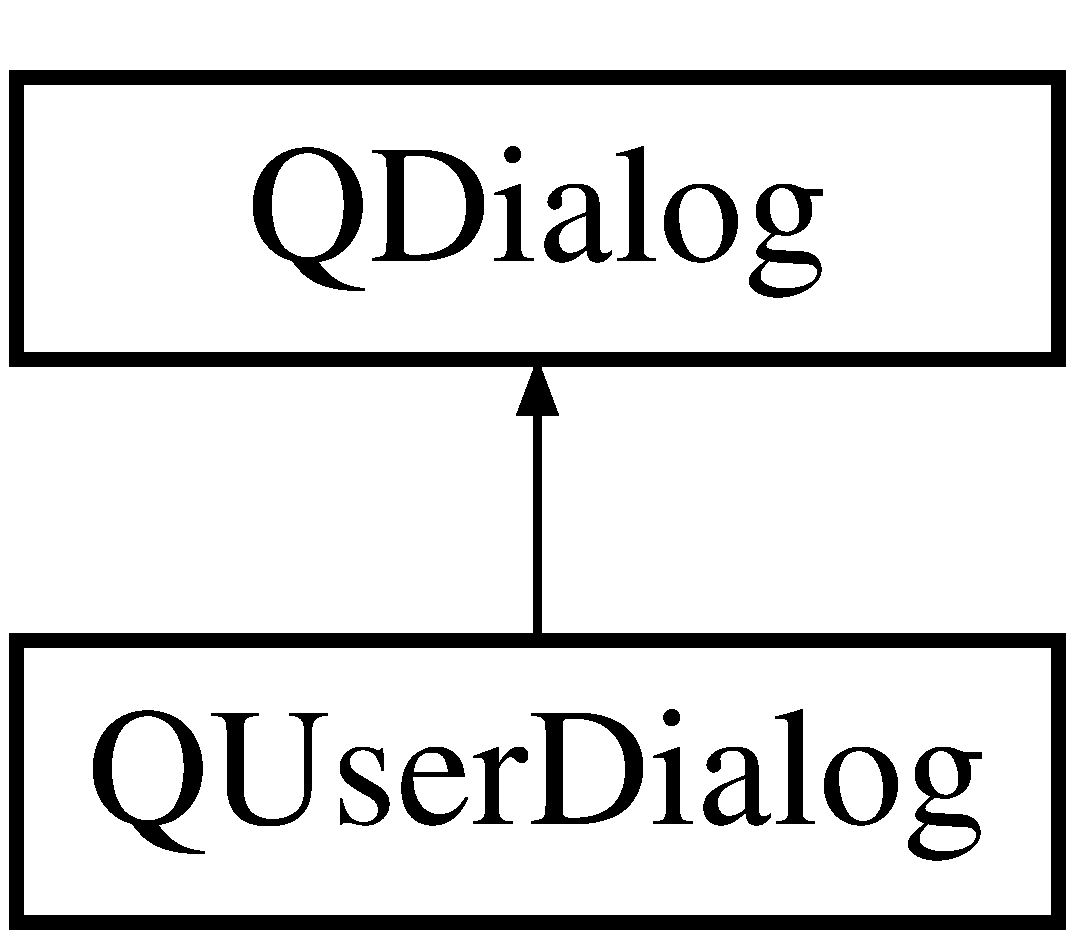
\includegraphics[height=2.000000cm]{classQUserDialog}
\end{center}
\end{figure}
\subsection*{Public Slots}
\begin{DoxyCompactItemize}
\item 
\hypertarget{classQUserDialog_ab8a9714ab638d850404417ed557bc45b}{void {\bfseries button\+Select} ()}\label{classQUserDialog_ab8a9714ab638d850404417ed557bc45b}

\item 
\hypertarget{classQUserDialog_a5028dd340b6debc4e5e4f796b781424e}{void {\bfseries button\+Create} ()}\label{classQUserDialog_a5028dd340b6debc4e5e4f796b781424e}

\end{DoxyCompactItemize}
\subsection*{Signals}
\begin{DoxyCompactItemize}
\item 
\hypertarget{classQUserDialog_a52d586a04c6b84f861ed6a143a606392}{void {\bfseries selected} (int index)}\label{classQUserDialog_a52d586a04c6b84f861ed6a143a606392}

\item 
\hypertarget{classQUserDialog_a12a528506faa30792c940725ac92ba72}{void {\bfseries done\+Event} (int r)}\label{classQUserDialog_a12a528506faa30792c940725ac92ba72}

\end{DoxyCompactItemize}
\subsection*{Public Member Functions}
\begin{DoxyCompactItemize}
\item 
\hypertarget{classQUserDialog_a120f5381a4a037acb2de11a49aa46e3e}{{\bfseries Q\+User\+Dialog} (const Q\+String\+List \&user\+List, Q\+Widget $\ast$parent=0)}\label{classQUserDialog_a120f5381a4a037acb2de11a49aa46e3e}

\item 
\hypertarget{classQUserDialog_ae1cff90bf82a90ad1f11947a59f02e82}{{\bfseries Q\+User\+Dialog} (Q\+Widget $\ast$parent=0)}\label{classQUserDialog_ae1cff90bf82a90ad1f11947a59f02e82}

\end{DoxyCompactItemize}


The documentation for this class was generated from the following files\+:\begin{DoxyCompactItemize}
\item 
view/quserdialog.\+h\item 
view/quserdialog.\+cpp\end{DoxyCompactItemize}

\hypertarget{classQUVChoisie}{\section{Q\+U\+V\+Choisie Class Reference}
\label{classQUVChoisie}\index{Q\+U\+V\+Choisie@{Q\+U\+V\+Choisie}}
}
Inheritance diagram for Q\+U\+V\+Choisie\+:\begin{figure}[H]
\begin{center}
\leavevmode
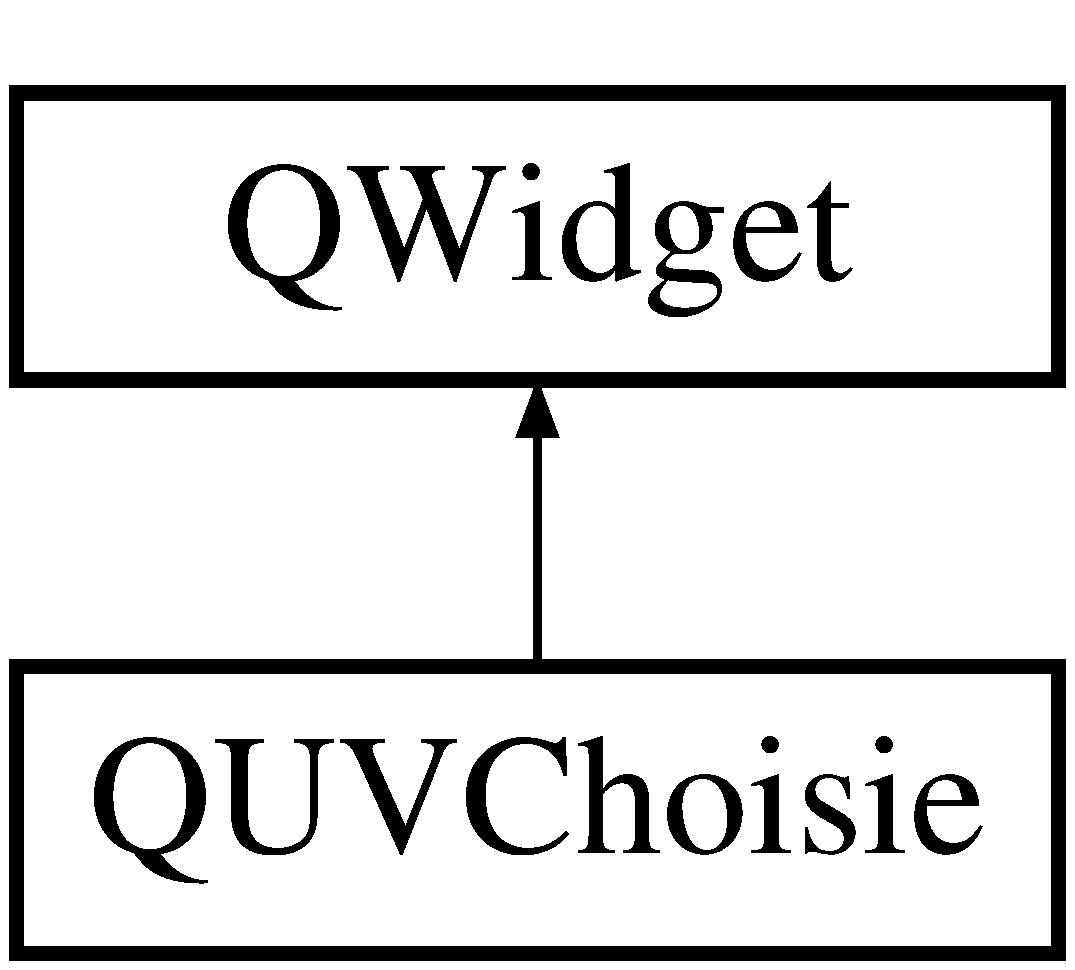
\includegraphics[height=2.000000cm]{classQUVChoisie}
\end{center}
\end{figure}
\subsection*{Public Slots}
\begin{DoxyCompactItemize}
\item 
\hypertarget{classQUVChoisie_a1bc7d18797b56c312082bb42b9350347}{void {\bfseries button\+Remove\+Clicked} ()}\label{classQUVChoisie_a1bc7d18797b56c312082bb42b9350347}

\item 
\hypertarget{classQUVChoisie_a04be97b4d99c43f5104762b3734894de}{void {\bfseries combo\+Note\+Changed} (Q\+String)}\label{classQUVChoisie_a04be97b4d99c43f5104762b3734894de}

\end{DoxyCompactItemize}
\subsection*{Signals}
\begin{DoxyCompactItemize}
\item 
\hypertarget{classQUVChoisie_aab80ca6e42ae0ee0e1404b1aab4cf758}{void {\bfseries remove\+Clicked} ()}\label{classQUVChoisie_aab80ca6e42ae0ee0e1404b1aab4cf758}

\item 
\hypertarget{classQUVChoisie_add5b9f406168959c0977dad304f4fcc2}{void {\bfseries note\+Changed} (Q\+String)}\label{classQUVChoisie_add5b9f406168959c0977dad304f4fcc2}

\end{DoxyCompactItemize}
\subsection*{Public Member Functions}
\begin{DoxyCompactItemize}
\item 
\hypertarget{classQUVChoisie_a248f74ec663eac3a1b40e188f248e365}{{\bfseries Q\+U\+V\+Choisie} (Q\+Widget $\ast$parent=0)}\label{classQUVChoisie_a248f74ec663eac3a1b40e188f248e365}

\item 
\hypertarget{classQUVChoisie_ae06021ab0da36bbd9318b26335e42593}{void {\bfseries set\+Name} (Q\+String s)}\label{classQUVChoisie_ae06021ab0da36bbd9318b26335e42593}

\item 
\hypertarget{classQUVChoisie_aa52a1e48864259c554ff01cb1e3ca6d6}{void {\bfseries set\+Note} (Q\+String note)}\label{classQUVChoisie_aa52a1e48864259c554ff01cb1e3ca6d6}

\item 
\hypertarget{classQUVChoisie_a6f3d77878a1a3f7d0064872fb328551c}{void {\bfseries add\+Notes} (Q\+String\+List notes)}\label{classQUVChoisie_a6f3d77878a1a3f7d0064872fb328551c}

\end{DoxyCompactItemize}


The documentation for this class was generated from the following files\+:\begin{DoxyCompactItemize}
\item 
view/quvchoisie.\+h\item 
view/quvchoisie.\+cpp\end{DoxyCompactItemize}

\hypertarget{classQUVListItemModel}{\section{Q\+U\+V\+List\+Item\+Model Class Reference}
\label{classQUVListItemModel}\index{Q\+U\+V\+List\+Item\+Model@{Q\+U\+V\+List\+Item\+Model}}
}
Inheritance diagram for Q\+U\+V\+List\+Item\+Model\+:\begin{figure}[H]
\begin{center}
\leavevmode
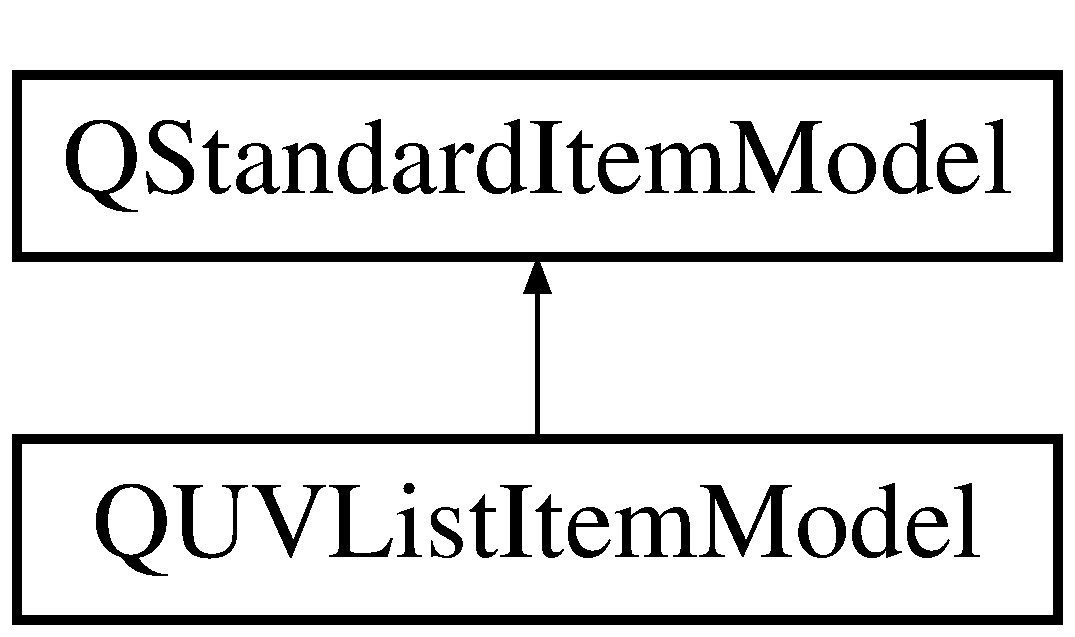
\includegraphics[height=2.000000cm]{classQUVListItemModel}
\end{center}
\end{figure}
\subsection*{Public Member Functions}
\begin{DoxyCompactItemize}
\item 
\hypertarget{classQUVListItemModel_af5d794524ca6e123a8173d988f89e3f8}{{\bfseries Q\+U\+V\+List\+Item\+Model} (Q\+Object $\ast$parent=0)}\label{classQUVListItemModel_af5d794524ca6e123a8173d988f89e3f8}

\end{DoxyCompactItemize}


The documentation for this class was generated from the following files\+:\begin{DoxyCompactItemize}
\item 
controller/quvlistitemmodel.\+h\item 
controller/quvlistitemmodel.\+cpp\end{DoxyCompactItemize}

\hypertarget{classQUVPreview}{\section{Q\+U\+V\+Preview Class Reference}
\label{classQUVPreview}\index{Q\+U\+V\+Preview@{Q\+U\+V\+Preview}}
}
Inheritance diagram for Q\+U\+V\+Preview\+:\begin{figure}[H]
\begin{center}
\leavevmode
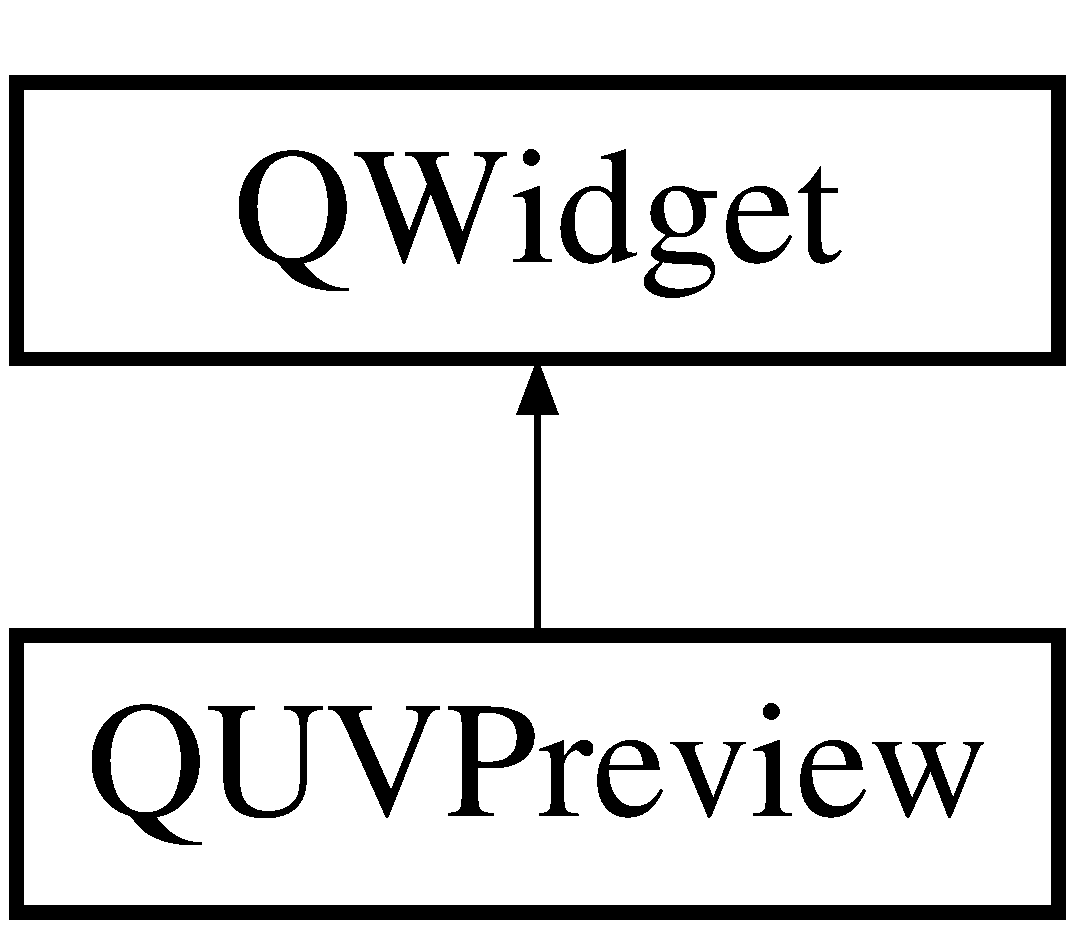
\includegraphics[height=2.000000cm]{classQUVPreview}
\end{center}
\end{figure}
\subsection*{Public Member Functions}
\begin{DoxyCompactItemize}
\item 
\hypertarget{classQUVPreview_af529e4c875911a5a652a306b41cda879}{{\bfseries Q\+U\+V\+Preview} (Q\+Widget $\ast$parent=0)}\label{classQUVPreview_af529e4c875911a5a652a306b41cda879}

\end{DoxyCompactItemize}


The documentation for this class was generated from the following files\+:\begin{DoxyCompactItemize}
\item 
view/quvpreview.\+h\item 
view/quvpreview.\+cpp\end{DoxyCompactItemize}

\hypertarget{classSemestre}{\section{Semestre Class Reference}
\label{classSemestre}\index{Semestre@{Semestre}}
}
Inheritance diagram for Semestre\+:\begin{figure}[H]
\begin{center}
\leavevmode
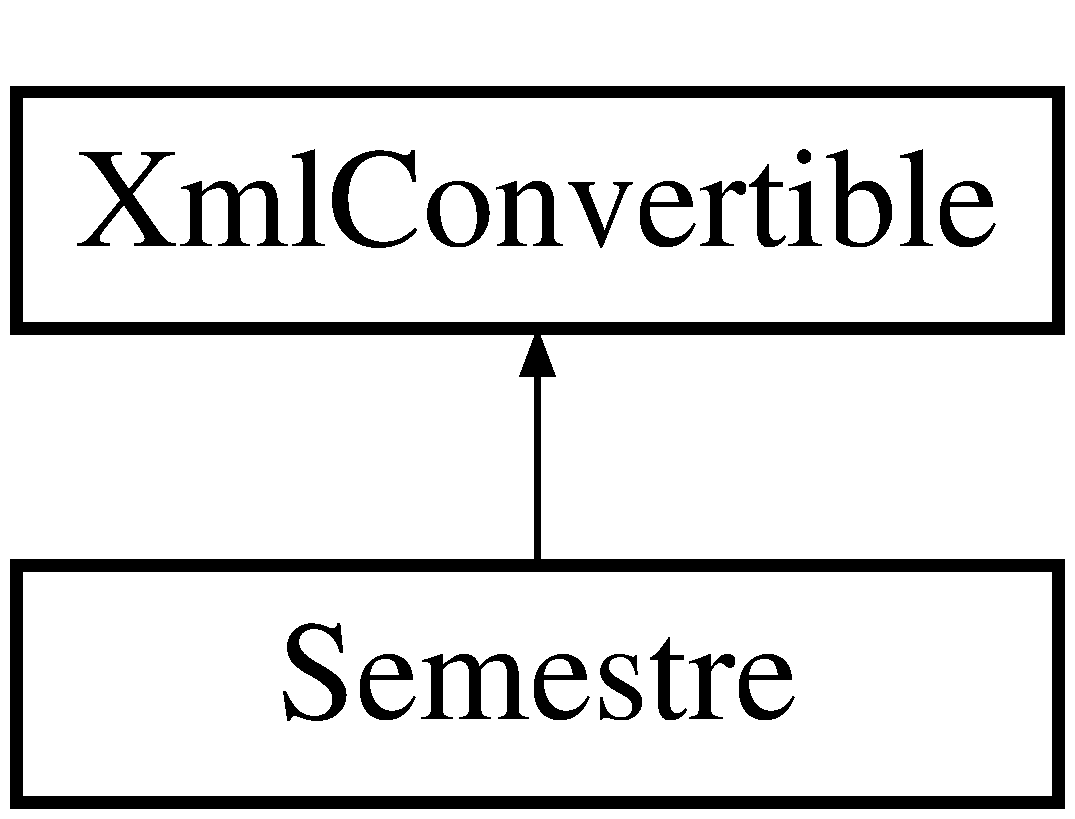
\includegraphics[height=2.000000cm]{classSemestre}
\end{center}
\end{figure}
\subsection*{Public Types}
\begin{DoxyCompactItemize}
\item 
\hypertarget{classSemestre_a1f4bcf95773a68fb7538c01c11a8cd7e}{enum {\bfseries Saison} \{ {\bfseries P\+R\+I\+N\+T\+E\+M\+P\+S}, 
{\bfseries A\+U\+T\+O\+M\+N\+E}
 \}}\label{classSemestre_a1f4bcf95773a68fb7538c01c11a8cd7e}

\end{DoxyCompactItemize}
\subsection*{Public Member Functions}
\begin{DoxyCompactItemize}
\item 
void \hyperlink{classSemestre_a4315bab4b2425a4000da60d3afb811e2}{ajouter\+Uv} (\hyperlink{classUVEtudiant}{U\+V\+Etudiant} $\ast$uv)
\begin{DoxyCompactList}\small\item\em Ajoute une uv au semestre. \end{DoxyCompactList}\item 
void \hyperlink{classSemestre_abb29a3e06f99052e28356a671c200c91}{supprimer\+Uv} (const Q\+String \&tag)
\begin{DoxyCompactList}\small\item\em Supprime une uv du semestre. \end{DoxyCompactList}\item 
\hypertarget{classSemestre_a9f63fd844fd580c26b7df6f3786bc59b}{void \hyperlink{classSemestre_a9f63fd844fd580c26b7df6f3786bc59b}{from\+Xml} (const Q\+Dom\+Node \&noeud)}\label{classSemestre_a9f63fd844fd580c26b7df6f3786bc59b}

\begin{DoxyCompactList}\small\item\em Définit l'objet à partir d'un élément X\+M\+L. \end{DoxyCompactList}\item 
Q\+Dom\+Element \hyperlink{classSemestre_a36272015189e8641d0a736f99981b876}{to\+Xml} () const 
\begin{DoxyCompactList}\small\item\em Convertit l'objet au format X\+M\+L. \end{DoxyCompactList}\item 
\hypertarget{classSemestre_adae6581e8bc96ed833939ba6d9ac62d8}{Q\+Map$<$ Q\+String, \hyperlink{classUVEtudiant}{U\+V\+Etudiant} $\ast$ $>$ {\bfseries uvs} () const }\label{classSemestre_adae6581e8bc96ed833939ba6d9ac62d8}

\item 
\hypertarget{classSemestre_ae829aa152161807619e874b98327f896}{int {\bfseries id} () const }\label{classSemestre_ae829aa152161807619e874b98327f896}

\item 
\hypertarget{classSemestre_aec76232f9da3b2e52947a403d426a8f2}{Q\+String {\bfseries nom} () const }\label{classSemestre_aec76232f9da3b2e52947a403d426a8f2}

\item 
\hypertarget{classSemestre_a0710500a4eafae6e30ef828b12768090}{enum Saison {\bfseries saison} () const }\label{classSemestre_a0710500a4eafae6e30ef828b12768090}

\item 
\hypertarget{classSemestre_a1828329d5f1aafef07a1f2756cf4d497}{int {\bfseries annee} () const }\label{classSemestre_a1828329d5f1aafef07a1f2756cf4d497}

\item 
\hypertarget{classSemestre_a3549ba8bcd42de751312150964f140cb}{void {\bfseries nom} (const Q\+String \&n)}\label{classSemestre_a3549ba8bcd42de751312150964f140cb}

\item 
\hypertarget{classSemestre_a2d106ad925696688381ca0e40ffca2b0}{void {\bfseries annee} (int a)}\label{classSemestre_a2d106ad925696688381ca0e40ffca2b0}

\item 
\hypertarget{classSemestre_ac851dbab40163f804a4a382faab38e23}{void {\bfseries saison} (enum Saison s)}\label{classSemestre_ac851dbab40163f804a4a382faab38e23}

\end{DoxyCompactItemize}
\subsection*{Static Public Attributes}
\begin{DoxyCompactItemize}
\item 
\hypertarget{classSemestre_a03fcd2d2eecdcaabfd6048473798f133}{static const Q\+String \hyperlink{classSemestre_a03fcd2d2eecdcaabfd6048473798f133}{X\+M\+L\+\_\+\+N\+O\+D\+E\+\_\+\+N\+A\+M\+E} = \char`\"{}semestre\char`\"{}}\label{classSemestre_a03fcd2d2eecdcaabfd6048473798f133}

\begin{DoxyCompactList}\small\item\em Nom du noeud X\+M\+L correspondant à un semestre. \end{DoxyCompactList}\end{DoxyCompactItemize}


\subsection{Member Function Documentation}
\hypertarget{classSemestre_a4315bab4b2425a4000da60d3afb811e2}{\index{Semestre@{Semestre}!ajouter\+Uv@{ajouter\+Uv}}
\index{ajouter\+Uv@{ajouter\+Uv}!Semestre@{Semestre}}
\subsubsection[{ajouter\+Uv}]{\setlength{\rightskip}{0pt plus 5cm}void Semestre\+::ajouter\+Uv (
\begin{DoxyParamCaption}
\item[{{\bf U\+V\+Etudiant} $\ast$}]{uv}
\end{DoxyParamCaption}
)}}\label{classSemestre_a4315bab4b2425a4000da60d3afb811e2}


Ajoute une uv au semestre. 


\begin{DoxyParams}{Parameters}
{\em uv} & L'uv à ajouter \\
\hline
\end{DoxyParams}
\hypertarget{classSemestre_abb29a3e06f99052e28356a671c200c91}{\index{Semestre@{Semestre}!supprimer\+Uv@{supprimer\+Uv}}
\index{supprimer\+Uv@{supprimer\+Uv}!Semestre@{Semestre}}
\subsubsection[{supprimer\+Uv}]{\setlength{\rightskip}{0pt plus 5cm}void Semestre\+::supprimer\+Uv (
\begin{DoxyParamCaption}
\item[{const Q\+String \&}]{tag}
\end{DoxyParamCaption}
)}}\label{classSemestre_abb29a3e06f99052e28356a671c200c91}


Supprime une uv du semestre. 


\begin{DoxyParams}{Parameters}
{\em tag} & Le tag de l'uv à supprimer \\
\hline
\end{DoxyParams}
\hypertarget{classSemestre_a36272015189e8641d0a736f99981b876}{\index{Semestre@{Semestre}!to\+Xml@{to\+Xml}}
\index{to\+Xml@{to\+Xml}!Semestre@{Semestre}}
\subsubsection[{to\+Xml}]{\setlength{\rightskip}{0pt plus 5cm}Q\+Dom\+Element Semestre\+::to\+Xml (
\begin{DoxyParamCaption}
{}
\end{DoxyParamCaption}
) const\hspace{0.3cm}{\ttfamily [virtual]}}}\label{classSemestre_a36272015189e8641d0a736f99981b876}


Convertit l'objet au format X\+M\+L. 

\begin{DoxyReturn}{Returns}
L'élément X\+M\+L correspondant 
\end{DoxyReturn}


Implements \hyperlink{classXmlConvertible_a188430d1503cf6db7223374306577c2c}{Xml\+Convertible}.



The documentation for this class was generated from the following files\+:\begin{DoxyCompactItemize}
\item 
model/semestre.\+h\item 
model/semestre.\+cpp\end{DoxyCompactItemize}

\hypertarget{classSemestreController}{\section{Semestre\+Controller Class Reference}
\label{classSemestreController}\index{Semestre\+Controller@{Semestre\+Controller}}
}
Inheritance diagram for Semestre\+Controller\+:\begin{figure}[H]
\begin{center}
\leavevmode
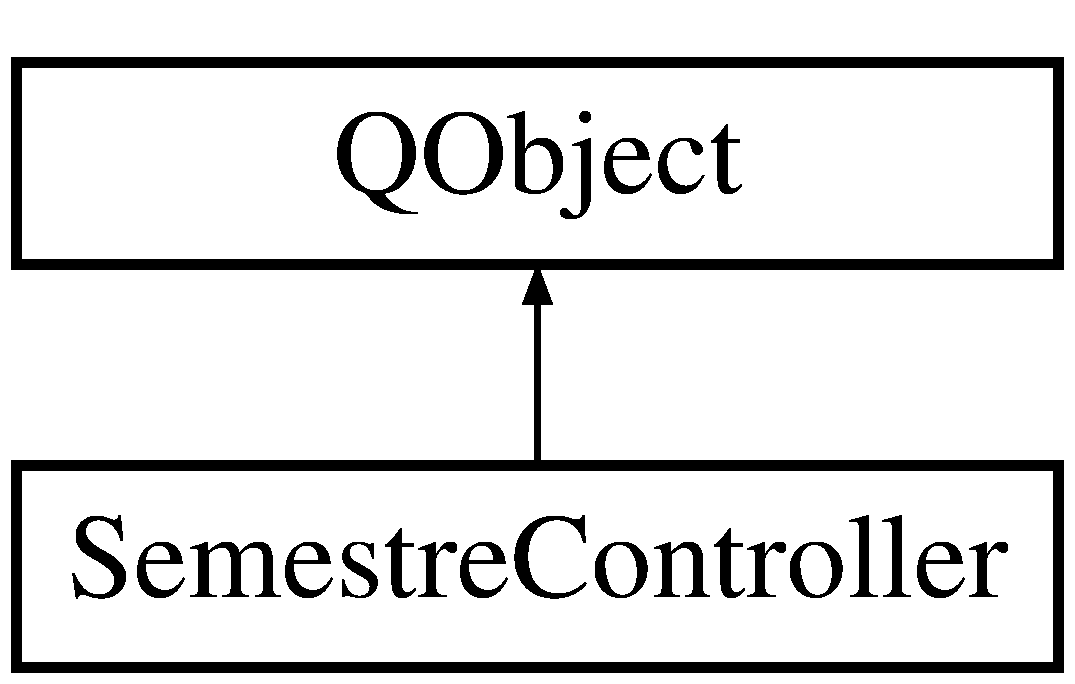
\includegraphics[height=2.000000cm]{classSemestreController}
\end{center}
\end{figure}
\subsection*{Public Slots}
\begin{DoxyCompactItemize}
\item 
\hypertarget{classSemestreController_a1bf45d14d271656c9757928365bb265a}{void {\bfseries remove} ()}\label{classSemestreController_a1bf45d14d271656c9757928365bb265a}

\item 
\hypertarget{classSemestreController_aa39c752c66b547f2416aad35927f7e4c}{void {\bfseries edit} ()}\label{classSemestreController_aa39c752c66b547f2416aad35927f7e4c}

\item 
\hypertarget{classSemestreController_a0667966f3c30e4e9860cd698ddced399}{void {\bfseries update} ()}\label{classSemestreController_a0667966f3c30e4e9860cd698ddced399}

\end{DoxyCompactItemize}
\subsection*{Signals}
\begin{DoxyCompactItemize}
\item 
\hypertarget{classSemestreController_a0b70f5ed336d6332b909583e2ce7dbdf}{void {\bfseries removed} (\hyperlink{classSemestre}{Semestre} $\ast$formation)}\label{classSemestreController_a0b70f5ed336d6332b909583e2ce7dbdf}

\item 
\hypertarget{classSemestreController_adee6430a8ff41583d14ae5a7add99512}{void {\bfseries \+\_\+removed} ()}\label{classSemestreController_adee6430a8ff41583d14ae5a7add99512}

\end{DoxyCompactItemize}
\subsection*{Public Member Functions}
\begin{DoxyCompactItemize}
\item 
\hypertarget{classSemestreController_aa1dc83e3ab722ce31841aad950882045}{{\bfseries Semestre\+Controller} (\hyperlink{classEtudiant}{Etudiant} $\ast$etudiant, \hyperlink{classSemestre}{Semestre} $\ast$semestre, \hyperlink{classQSemestre}{Q\+Semestre} $\ast$q\+Semestre, Q\+Object $\ast$parent=0)}\label{classSemestreController_aa1dc83e3ab722ce31841aad950882045}

\end{DoxyCompactItemize}


The documentation for this class was generated from the following files\+:\begin{DoxyCompactItemize}
\item 
controller/semestrecontroller.\+h\item 
controller/semestrecontroller.\+cpp\end{DoxyCompactItemize}

\hypertarget{classSemestreDialogController}{\section{Semestre\+Dialog\+Controller Class Reference}
\label{classSemestreDialogController}\index{Semestre\+Dialog\+Controller@{Semestre\+Dialog\+Controller}}
}
Inheritance diagram for Semestre\+Dialog\+Controller\+:\begin{figure}[H]
\begin{center}
\leavevmode
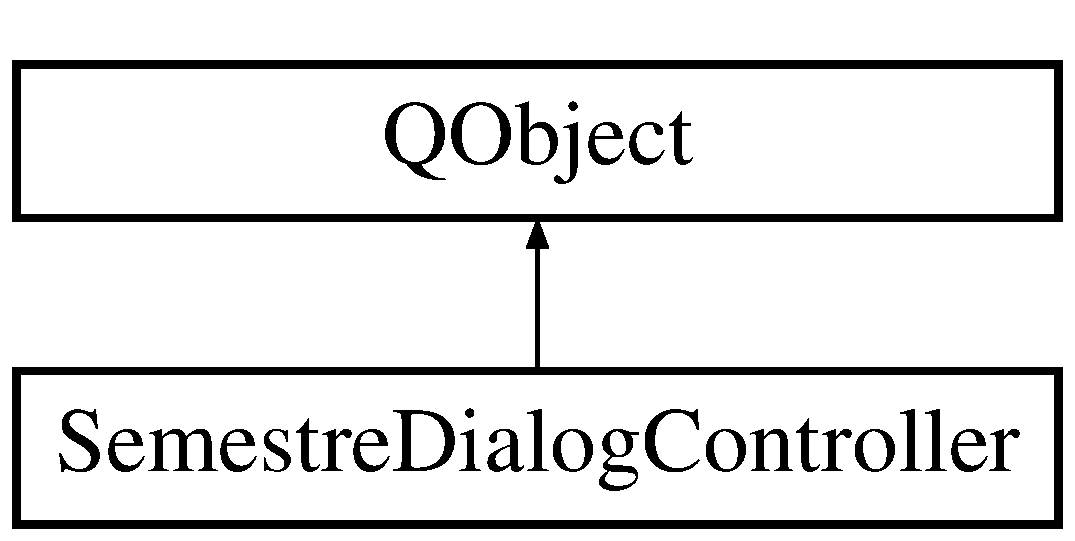
\includegraphics[height=2.000000cm]{classSemestreDialogController}
\end{center}
\end{figure}
\subsection*{Public Slots}
\begin{DoxyCompactItemize}
\item 
\hypertarget{classSemestreDialogController_a925085e9a56ae23743c0847311edc0b9}{void {\bfseries update} ()}\label{classSemestreDialogController_a925085e9a56ae23743c0847311edc0b9}

\item 
\hypertarget{classSemestreDialogController_abf99701af29111884c4c20176b2c2a32}{void {\bfseries uv\+Choisie\+Removed} (\hyperlink{classUVEtudiant}{U\+V\+Etudiant} $\ast$uv)}\label{classSemestreDialogController_abf99701af29111884c4c20176b2c2a32}

\item 
\hypertarget{classSemestreDialogController_ab3492ad04f1f7593e724b154a5d4e52b}{void {\bfseries saison\+Changed} ()}\label{classSemestreDialogController_ab3492ad04f1f7593e724b154a5d4e52b}

\item 
\hypertarget{classSemestreDialogController_a04840096badb41896bb5e902bc3576c4}{void {\bfseries year\+Changed} (int year)}\label{classSemestreDialogController_a04840096badb41896bb5e902bc3576c4}

\item 
\hypertarget{classSemestreDialogController_aa59e7840988eea5818109c98f8eafac4}{void {\bfseries filter\+Changed} (Q\+String\+List list)}\label{classSemestreDialogController_aa59e7840988eea5818109c98f8eafac4}

\end{DoxyCompactItemize}
\subsection*{Signals}
\begin{DoxyCompactItemize}
\item 
\hypertarget{classSemestreDialogController_a42eebeffab549104cfc7c3e34b579344}{void {\bfseries updated} ()}\label{classSemestreDialogController_a42eebeffab549104cfc7c3e34b579344}

\end{DoxyCompactItemize}
\subsection*{Public Member Functions}
\begin{DoxyCompactItemize}
\item 
\hypertarget{classSemestreDialogController_adf3bc854ee99e2701a186f599a632cb6}{{\bfseries Semestre\+Dialog\+Controller} (\hyperlink{classEtudiant}{Etudiant} $\ast$etudiant, \hyperlink{classSemestre}{Semestre} $\ast$semestre, Q\+Object $\ast$parent=0)}\label{classSemestreDialogController_adf3bc854ee99e2701a186f599a632cb6}

\end{DoxyCompactItemize}


The documentation for this class was generated from the following files\+:\begin{DoxyCompactItemize}
\item 
controller/semestredialogcontroller.\+h\item 
controller/semestredialogcontroller.\+cpp\end{DoxyCompactItemize}

\hypertarget{classsemestreInvalideErreur}{\section{semestre\+Invalide\+Erreur Class Reference}
\label{classsemestreInvalideErreur}\index{semestre\+Invalide\+Erreur@{semestre\+Invalide\+Erreur}}
}
Inheritance diagram for semestre\+Invalide\+Erreur\+:\begin{figure}[H]
\begin{center}
\leavevmode
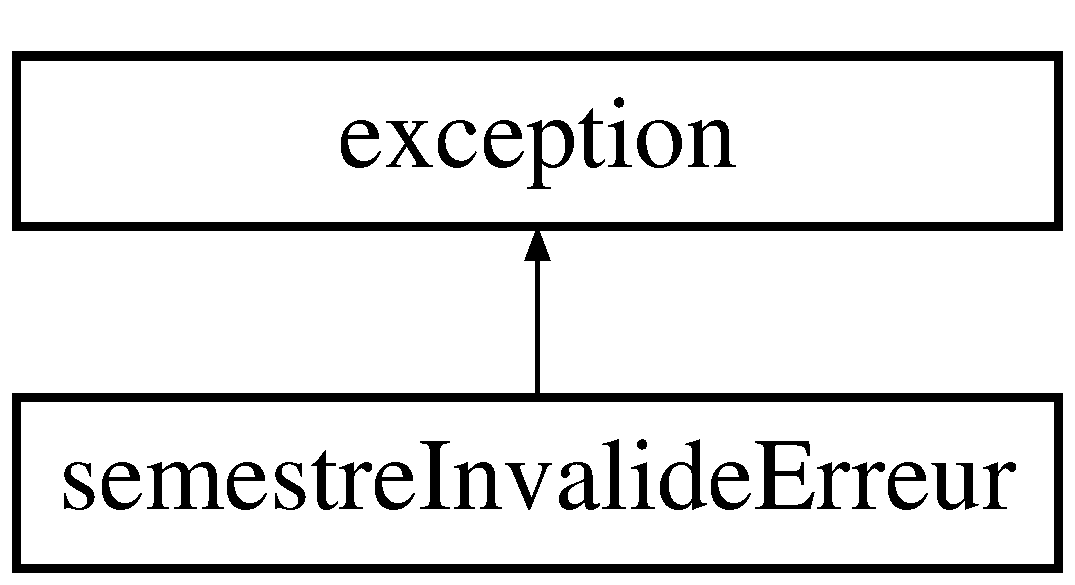
\includegraphics[height=2.000000cm]{classsemestreInvalideErreur}
\end{center}
\end{figure}
\subsection*{Public Member Functions}
\begin{DoxyCompactItemize}
\item 
\hypertarget{classsemestreInvalideErreur_a84f8fe270c828d40c338ea49833493f0}{{\bfseries semestre\+Invalide\+Erreur} (Q\+List$<$ \hyperlink{classUVEtudiant}{U\+V\+Etudiant} $>$ \&deja\+Validees)}\label{classsemestreInvalideErreur_a84f8fe270c828d40c338ea49833493f0}

\item 
\hypertarget{classsemestreInvalideErreur_a4b6dc1768e3d16456f18ec33384ec761}{virtual const char $\ast$ {\bfseries what} () const   throw ()}\label{classsemestreInvalideErreur_a4b6dc1768e3d16456f18ec33384ec761}

\item 
\hypertarget{classsemestreInvalideErreur_a2f289558801d7de1038a99a636138139}{Q\+List$<$ \hyperlink{classUVEtudiant}{U\+V\+Etudiant} $>$ {\bfseries deja\+Validees} () const }\label{classsemestreInvalideErreur_a2f289558801d7de1038a99a636138139}

\end{DoxyCompactItemize}


The documentation for this class was generated from the following file\+:\begin{DoxyCompactItemize}
\item 
model/semestre\+Invalide\+Erreur.\+h\end{DoxyCompactItemize}

\hypertarget{classUV}{\section{U\+V Class Reference}
\label{classUV}\index{U\+V@{U\+V}}
}
Inheritance diagram for U\+V\+:\begin{figure}[H]
\begin{center}
\leavevmode
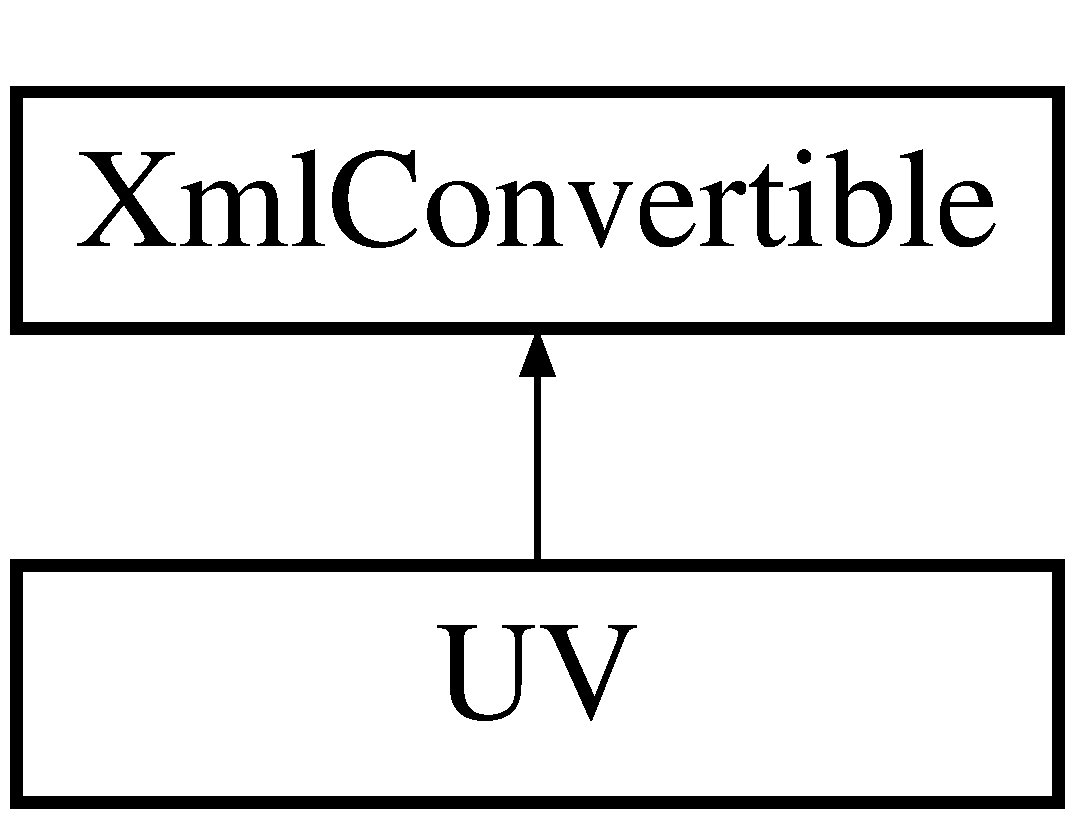
\includegraphics[height=2.000000cm]{classUV}
\end{center}
\end{figure}
\subsection*{Public Member Functions}
\begin{DoxyCompactItemize}
\item 
\hypertarget{classUV_a189e0eb0552c048eec21c2f37e49dc4b}{void \hyperlink{classUV_a189e0eb0552c048eec21c2f37e49dc4b}{from\+Xml} (const Q\+Dom\+Node \&noeud)}\label{classUV_a189e0eb0552c048eec21c2f37e49dc4b}

\begin{DoxyCompactList}\small\item\em Définit l'objet à partir d'un élément X\+M\+L. \end{DoxyCompactList}\item 
Q\+Dom\+Element \hyperlink{classUV_a2b60d0325f1117f3228f8ff32667e860}{to\+Xml} () const 
\begin{DoxyCompactList}\small\item\em Convertit l'objet au format X\+M\+L. \end{DoxyCompactList}\item 
\hypertarget{classUV_a32444f5089aad36c217b2c4de6a7ee65}{Q\+String {\bfseries tag} () const }\label{classUV_a32444f5089aad36c217b2c4de6a7ee65}

\item 
\hypertarget{classUV_ae88e929ca287f9b997ccffeaefba1344}{Q\+String {\bfseries titre} () const }\label{classUV_ae88e929ca287f9b997ccffeaefba1344}

\item 
\hypertarget{classUV_a8a384525c3ab6c316393cbee86bcdf6f}{Q\+String\+List {\bfseries cursus} () const }\label{classUV_a8a384525c3ab6c316393cbee86bcdf6f}

\item 
\hypertarget{classUV_a4b8c342724e30ea587ba15b914b741e5}{bool {\bfseries automne} () const }\label{classUV_a4b8c342724e30ea587ba15b914b741e5}

\item 
\hypertarget{classUV_ad81328803813c7197f959a42984485bc}{bool {\bfseries printemps} () const }\label{classUV_ad81328803813c7197f959a42984485bc}

\item 
\hypertarget{classUV_acff84ec643c8bdf7e30c0837f61ada14}{Q\+Map$<$ Q\+String, unsigned int $>$ {\bfseries credits} () const }\label{classUV_acff84ec643c8bdf7e30c0837f61ada14}

\item 
\hypertarget{classUV_ab450823845332c36d69c1896dc4f9f58}{void {\bfseries tag} (Q\+String t)}\label{classUV_ab450823845332c36d69c1896dc4f9f58}

\item 
\hypertarget{classUV_a27b848bf182243f1620ccaa4e919ea95}{void {\bfseries titre} (Q\+String d)}\label{classUV_a27b848bf182243f1620ccaa4e919ea95}

\item 
\hypertarget{classUV_adaf893cc83cc4fa8c0c6ba20a35d1a76}{void {\bfseries cursus} (const Q\+String\+List \&c)}\label{classUV_adaf893cc83cc4fa8c0c6ba20a35d1a76}

\item 
\hypertarget{classUV_af54b2e6bfc9ea527aa01ae6023057cad}{void {\bfseries automne} (bool a)}\label{classUV_af54b2e6bfc9ea527aa01ae6023057cad}

\item 
\hypertarget{classUV_ae861b75787135b56b3ee36b42bd45e37}{void {\bfseries printemps} (bool p)}\label{classUV_ae861b75787135b56b3ee36b42bd45e37}

\item 
\hypertarget{classUV_abf2d72f28de424d3d0d3df7fa339f869}{Q\+String {\bfseries to\+String} () const }\label{classUV_abf2d72f28de424d3d0d3df7fa339f869}

\end{DoxyCompactItemize}
\subsection*{Static Public Attributes}
\begin{DoxyCompactItemize}
\item 
\hypertarget{classUV_a3d0a7fd96f0bb15ad0e23365cec09e13}{static const Q\+String \hyperlink{classUV_a3d0a7fd96f0bb15ad0e23365cec09e13}{X\+M\+L\+\_\+\+N\+O\+D\+E\+\_\+\+N\+A\+M\+E} = \char`\"{}uv\char`\"{}}\label{classUV_a3d0a7fd96f0bb15ad0e23365cec09e13}

\begin{DoxyCompactList}\small\item\em Nom du noeud X\+M\+L correspondant à une uv. \end{DoxyCompactList}\item 
\hypertarget{classUV_afef2ca86c5d563602d2ef39a3a08841e}{static const Q\+String \hyperlink{classUV_afef2ca86c5d563602d2ef39a3a08841e}{C\+R\+E\+D\+I\+T\+\_\+\+X\+M\+L\+\_\+\+N\+O\+D\+E\+\_\+\+N\+A\+M\+E} = \char`\"{}credits\char`\"{}}\label{classUV_afef2ca86c5d563602d2ef39a3a08841e}

\begin{DoxyCompactList}\small\item\em Nom du noeud X\+M\+L correspondant aux crédits apportés par une uv pour une catégorie. \end{DoxyCompactList}\end{DoxyCompactItemize}


\subsection{Member Function Documentation}
\hypertarget{classUV_a2b60d0325f1117f3228f8ff32667e860}{\index{U\+V@{U\+V}!to\+Xml@{to\+Xml}}
\index{to\+Xml@{to\+Xml}!U\+V@{U\+V}}
\subsubsection[{to\+Xml}]{\setlength{\rightskip}{0pt plus 5cm}Q\+Dom\+Element U\+V\+::to\+Xml (
\begin{DoxyParamCaption}
{}
\end{DoxyParamCaption}
) const\hspace{0.3cm}{\ttfamily [virtual]}}}\label{classUV_a2b60d0325f1117f3228f8ff32667e860}


Convertit l'objet au format X\+M\+L. 

\begin{DoxyReturn}{Returns}
L'élément X\+M\+L correspondant 
\end{DoxyReturn}


Implements \hyperlink{classXmlConvertible_a188430d1503cf6db7223374306577c2c}{Xml\+Convertible}.



The documentation for this class was generated from the following files\+:\begin{DoxyCompactItemize}
\item 
model/uv.\+h\item 
model/uv.\+cpp\end{DoxyCompactItemize}

\hypertarget{classUVChoisieController}{\section{U\+V\+Choisie\+Controller Class Reference}
\label{classUVChoisieController}\index{U\+V\+Choisie\+Controller@{U\+V\+Choisie\+Controller}}
}
Inheritance diagram for U\+V\+Choisie\+Controller\+:\begin{figure}[H]
\begin{center}
\leavevmode
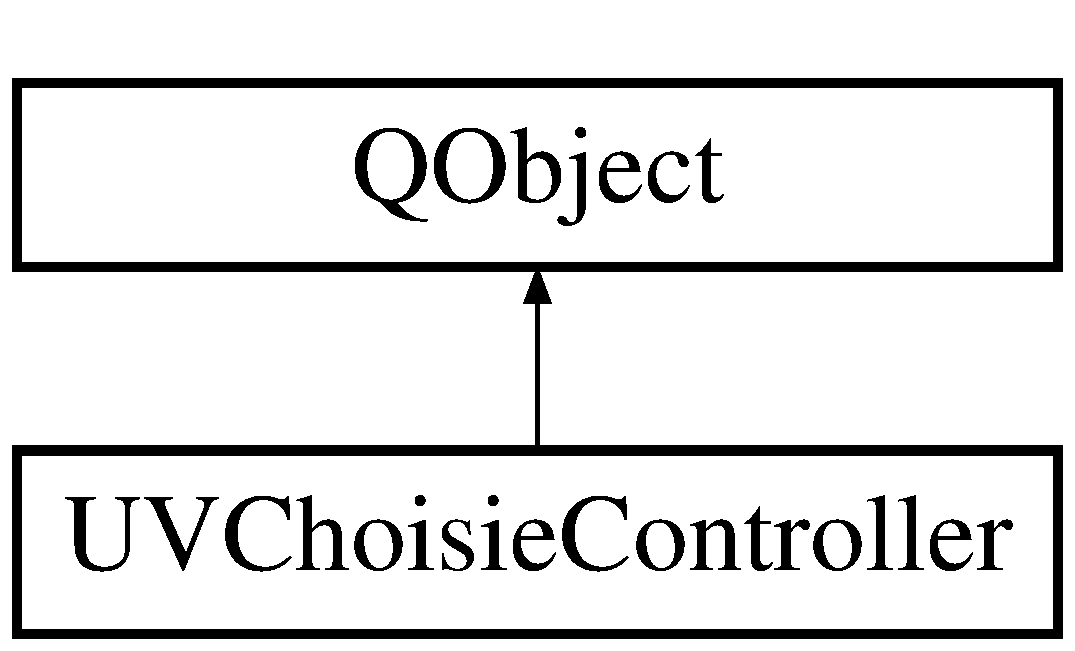
\includegraphics[height=2.000000cm]{classUVChoisieController}
\end{center}
\end{figure}
\subsection*{Public Slots}
\begin{DoxyCompactItemize}
\item 
\hypertarget{classUVChoisieController_a708375ad233a6733def4cacc29499a60}{void {\bfseries remove} ()}\label{classUVChoisieController_a708375ad233a6733def4cacc29499a60}

\item 
\hypertarget{classUVChoisieController_ad71f0a3a924a9e5751b0d1dbd13bd5d6}{void {\bfseries note\+Changed} (Q\+String note)}\label{classUVChoisieController_ad71f0a3a924a9e5751b0d1dbd13bd5d6}

\end{DoxyCompactItemize}
\subsection*{Signals}
\begin{DoxyCompactItemize}
\item 
\hypertarget{classUVChoisieController_abd99d85ee5e8ff0fae911b5577d1ee54}{void {\bfseries \+\_\+remove} ()}\label{classUVChoisieController_abd99d85ee5e8ff0fae911b5577d1ee54}

\item 
\hypertarget{classUVChoisieController_a12b646fc9ad01bb316f4cbc98eb8e4a1}{void {\bfseries removed} (\hyperlink{classUVEtudiant}{U\+V\+Etudiant} $\ast$)}\label{classUVChoisieController_a12b646fc9ad01bb316f4cbc98eb8e4a1}

\item 
\hypertarget{classUVChoisieController_a85ae65b9a0c88969439b85f80f36881d}{void {\bfseries updated} ()}\label{classUVChoisieController_a85ae65b9a0c88969439b85f80f36881d}

\end{DoxyCompactItemize}
\subsection*{Public Member Functions}
\begin{DoxyCompactItemize}
\item 
\hypertarget{classUVChoisieController_a110b8137e2dce05f0b2575f0f03c1598}{{\bfseries U\+V\+Choisie\+Controller} (\hyperlink{classUVEtudiant}{U\+V\+Etudiant} $\ast$uv, \hyperlink{classQUVChoisie}{Q\+U\+V\+Choisie} $\ast$uv\+Choisie, Q\+Object $\ast$parent=0)}\label{classUVChoisieController_a110b8137e2dce05f0b2575f0f03c1598}

\end{DoxyCompactItemize}


The documentation for this class was generated from the following files\+:\begin{DoxyCompactItemize}
\item 
controller/uvchoisiecontroller.\+h\item 
controller/uvchoisiecontroller.\+cpp\end{DoxyCompactItemize}

\hypertarget{classUVEtudiant}{\section{U\+V\+Etudiant Class Reference}
\label{classUVEtudiant}\index{U\+V\+Etudiant@{U\+V\+Etudiant}}
}
Inheritance diagram for U\+V\+Etudiant\+:\begin{figure}[H]
\begin{center}
\leavevmode
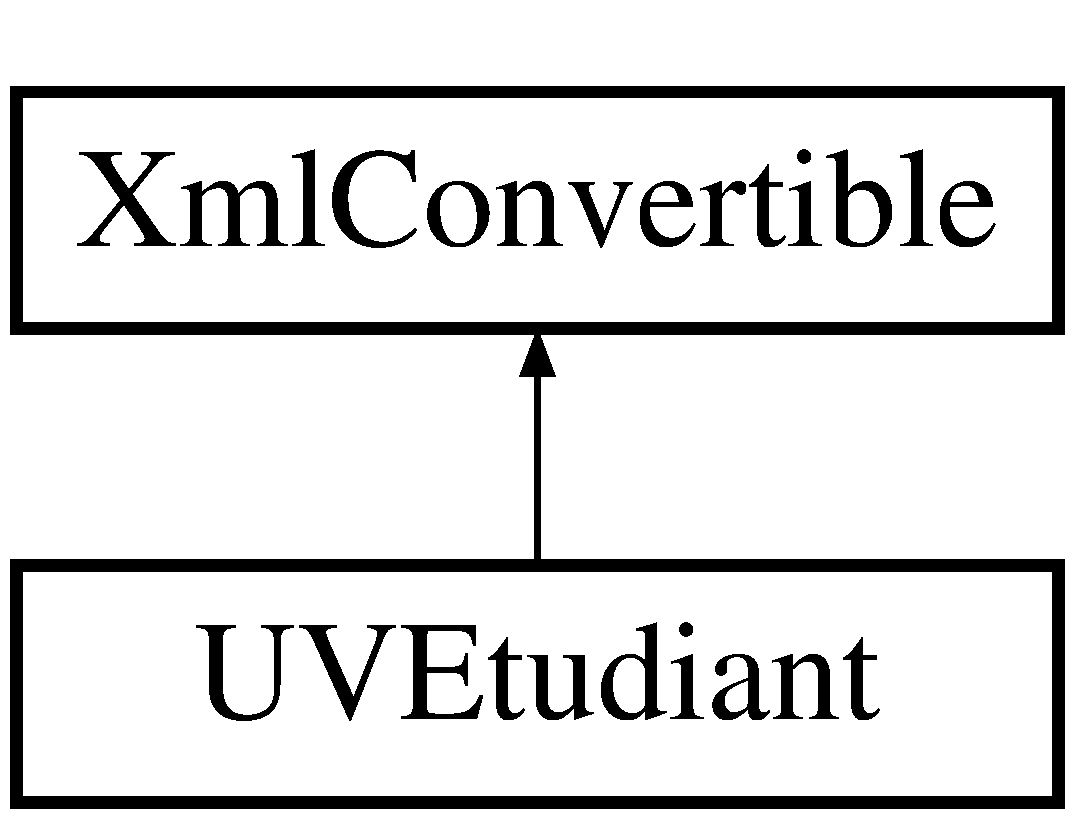
\includegraphics[height=2.000000cm]{classUVEtudiant}
\end{center}
\end{figure}
\subsection*{Public Member Functions}
\begin{DoxyCompactItemize}
\item 
\hypertarget{classUVEtudiant_adf59df3b1d84f30fa08018f00091f6bd}{{\bfseries U\+V\+Etudiant} (const \hyperlink{classUV}{U\+V} \&uv)}\label{classUVEtudiant_adf59df3b1d84f30fa08018f00091f6bd}

\item 
\hypertarget{classUVEtudiant_afc5de4526603bc33c6b8445b7297a896}{{\bfseries U\+V\+Etudiant} (const Q\+Dom\+Node \&node)}\label{classUVEtudiant_afc5de4526603bc33c6b8445b7297a896}

\item 
\hypertarget{classUVEtudiant_a704e657fa6cc2ec18b5d68028ed1cb75}{void \hyperlink{classUVEtudiant_a704e657fa6cc2ec18b5d68028ed1cb75}{from\+Xml} (const Q\+Dom\+Node \&noeud)}\label{classUVEtudiant_a704e657fa6cc2ec18b5d68028ed1cb75}

\begin{DoxyCompactList}\small\item\em Définit l'objet à partir d'un élément X\+M\+L. \end{DoxyCompactList}\item 
Q\+Dom\+Element \hyperlink{classUVEtudiant_a4a4aef90cdc3207ccab922d1b8b38334}{to\+Xml} () const 
\begin{DoxyCompactList}\small\item\em Convertit l'objet au format X\+M\+L. \end{DoxyCompactList}\item 
\hypertarget{classUVEtudiant_af9fbad2a00b76ad0201c503f9c2449be}{Q\+String {\bfseries tag} () const }\label{classUVEtudiant_af9fbad2a00b76ad0201c503f9c2449be}

\item 
\hypertarget{classUVEtudiant_a8c57efeab3b71714e931e54d4ac440e6}{Q\+String {\bfseries titre} () const }\label{classUVEtudiant_a8c57efeab3b71714e931e54d4ac440e6}

\item 
\hypertarget{classUVEtudiant_a7d336ff9eff012d1d4cd928e86d1fdf3}{Q\+String\+List {\bfseries cursus} () const }\label{classUVEtudiant_a7d336ff9eff012d1d4cd928e86d1fdf3}

\item 
\hypertarget{classUVEtudiant_a454e7e10ded3888b8bc139bbfc449465}{bool {\bfseries automne} () const }\label{classUVEtudiant_a454e7e10ded3888b8bc139bbfc449465}

\item 
\hypertarget{classUVEtudiant_a1cb9fee2119f5ac89cc0871929907f14}{bool {\bfseries printemps} () const }\label{classUVEtudiant_a1cb9fee2119f5ac89cc0871929907f14}

\item 
\hypertarget{classUVEtudiant_aa9e6688f67df51ddac6822d6181eb2c8}{Q\+Map$<$ Q\+String, unsigned int $>$ {\bfseries credits} () const }\label{classUVEtudiant_aa9e6688f67df51ddac6822d6181eb2c8}

\item 
\hypertarget{classUVEtudiant_ac04557b040457e811b3d29d8c412651c}{Q\+String {\bfseries note} () const }\label{classUVEtudiant_ac04557b040457e811b3d29d8c412651c}

\item 
\hypertarget{classUVEtudiant_a592fdb389dc7b53a26fe647a9802eea2}{void {\bfseries note} (const Q\+String \&n)}\label{classUVEtudiant_a592fdb389dc7b53a26fe647a9802eea2}

\end{DoxyCompactItemize}
\subsection*{Static Public Member Functions}
\begin{DoxyCompactItemize}
\item 
\hypertarget{classUVEtudiant_a65ad7b8c17cc2f86fdbc2410ec9f9c3d}{static Q\+List$<$ Q\+String $>$ {\bfseries liste\+Notes} ()}\label{classUVEtudiant_a65ad7b8c17cc2f86fdbc2410ec9f9c3d}

\end{DoxyCompactItemize}
\subsection*{Static Public Attributes}
\begin{DoxyCompactItemize}
\item 
\hypertarget{classUVEtudiant_aceb9273c412c32a5a95156974c1c83eb}{static const Q\+String \hyperlink{classUVEtudiant_aceb9273c412c32a5a95156974c1c83eb}{X\+M\+L\+\_\+\+N\+O\+D\+E\+\_\+\+N\+A\+M\+E} = \char`\"{}uv\char`\"{}}\label{classUVEtudiant_aceb9273c412c32a5a95156974c1c83eb}

\begin{DoxyCompactList}\small\item\em Nom du noeud X\+M\+L correspondant à une uv. \end{DoxyCompactList}\end{DoxyCompactItemize}


\subsection{Member Function Documentation}
\hypertarget{classUVEtudiant_a4a4aef90cdc3207ccab922d1b8b38334}{\index{U\+V\+Etudiant@{U\+V\+Etudiant}!to\+Xml@{to\+Xml}}
\index{to\+Xml@{to\+Xml}!U\+V\+Etudiant@{U\+V\+Etudiant}}
\subsubsection[{to\+Xml}]{\setlength{\rightskip}{0pt plus 5cm}Q\+Dom\+Element U\+V\+Etudiant\+::to\+Xml (
\begin{DoxyParamCaption}
{}
\end{DoxyParamCaption}
) const\hspace{0.3cm}{\ttfamily [virtual]}}}\label{classUVEtudiant_a4a4aef90cdc3207ccab922d1b8b38334}


Convertit l'objet au format X\+M\+L. 

\begin{DoxyReturn}{Returns}
L'élément X\+M\+L correspondant 
\end{DoxyReturn}


Implements \hyperlink{classXmlConvertible_a188430d1503cf6db7223374306577c2c}{Xml\+Convertible}.



The documentation for this class was generated from the following files\+:\begin{DoxyCompactItemize}
\item 
model/uv\+Etudiant.\+h\item 
model/uv\+Etudiant.\+cpp\end{DoxyCompactItemize}

\hypertarget{classXmlConvertible}{\section{Xml\+Convertible Class Reference}
\label{classXmlConvertible}\index{Xml\+Convertible@{Xml\+Convertible}}
}
Inheritance diagram for Xml\+Convertible\+:\begin{figure}[H]
\begin{center}
\leavevmode
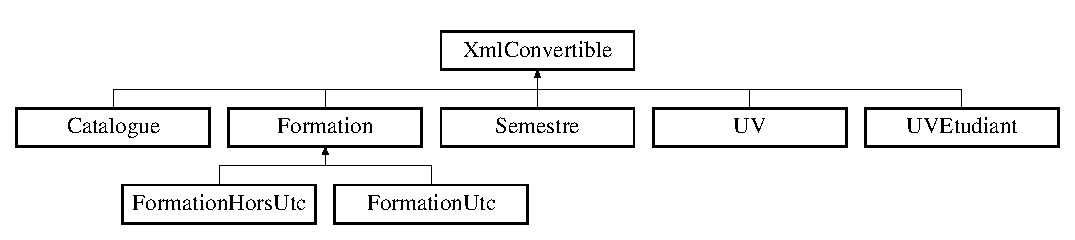
\includegraphics[height=2.776860cm]{classXmlConvertible}
\end{center}
\end{figure}
\subsection*{Public Member Functions}
\begin{DoxyCompactItemize}
\item 
virtual Q\+Dom\+Element \hyperlink{classXmlConvertible_a188430d1503cf6db7223374306577c2c}{to\+Xml} () const =0
\begin{DoxyCompactList}\small\item\em Convertit l'objet au format X\+M\+L. \end{DoxyCompactList}\item 
\hypertarget{classXmlConvertible_a269144f79b0b2c6aa1f7dd1993d94451}{virtual void \hyperlink{classXmlConvertible_a269144f79b0b2c6aa1f7dd1993d94451}{from\+Xml} (const Q\+Dom\+Node \&n)=0}\label{classXmlConvertible_a269144f79b0b2c6aa1f7dd1993d94451}

\begin{DoxyCompactList}\small\item\em Définit l'objet à partir d'un élément X\+M\+L. \end{DoxyCompactList}\end{DoxyCompactItemize}


\subsection{Member Function Documentation}
\hypertarget{classXmlConvertible_a188430d1503cf6db7223374306577c2c}{\index{Xml\+Convertible@{Xml\+Convertible}!to\+Xml@{to\+Xml}}
\index{to\+Xml@{to\+Xml}!Xml\+Convertible@{Xml\+Convertible}}
\subsubsection[{to\+Xml}]{\setlength{\rightskip}{0pt plus 5cm}virtual Q\+Dom\+Element Xml\+Convertible\+::to\+Xml (
\begin{DoxyParamCaption}
{}
\end{DoxyParamCaption}
) const\hspace{0.3cm}{\ttfamily [pure virtual]}}}\label{classXmlConvertible_a188430d1503cf6db7223374306577c2c}


Convertit l'objet au format X\+M\+L. 

\begin{DoxyReturn}{Returns}
L'élément X\+M\+L correspondant 
\end{DoxyReturn}


Implemented in \hyperlink{classCatalogue_a12f412e8ba3dd8b950fc1f7dd8608f51}{Catalogue}, \hyperlink{classUVEtudiant_a4a4aef90cdc3207ccab922d1b8b38334}{U\+V\+Etudiant}, \hyperlink{classFormation_aea1a12114f435bba6a32a0a32ca32e47}{Formation}, \hyperlink{classSemestre_a36272015189e8641d0a736f99981b876}{Semestre}, \hyperlink{classFormationUtc_a8dcda30820484cd00e82ad53a1b313f9}{Formation\+Utc}, \hyperlink{classFormationHorsUtc_ab7f0cb9fcecf0423b257d1011e7d8623}{Formation\+Hors\+Utc}, and \hyperlink{classUV_a2b60d0325f1117f3228f8ff32667e860}{U\+V}.



The documentation for this class was generated from the following file\+:\begin{DoxyCompactItemize}
\item 
model/xml\+Convertible.\+h\end{DoxyCompactItemize}

%--- End generated contents ---

% Index
\newpage
\phantomsection
\addcontentsline{toc}{chapter}{Index}
\printindex

\end{document}
